\documentclass[11pt,a4paper]{article}
\usepackage{fontspec}
\setmainfont{TeX Gyre Pagella}
\newfontfamily\headfont{Inter}[UprightFont=*-ExtraBold,BoldFont=*-ExtraBold,Extension=.otf,Path=/usr/share/fonts/opentype/inter/]
\usepackage[a4paper,margin=2.3cm]{geometry}
\usepackage{graphicx,booktabs,float,caption,array,xcolor}
\usepackage[hidelinks]{hyperref}
\usepackage{titlesec}
\usepackage[round]{natbib}
\usepackage{setspace}
\setstretch{1.05}
\renewcommand{\topfraction}{0.9}
\renewcommand{\bottomfraction}{0.8}
\renewcommand{\textfraction}{0.1}
\renewcommand{\floatpagefraction}{0.75}
\setlength{\parindent}{0pt}
\setlength{\parskip}{0.55em}
\titleformat{\section}{\headfont\Large}{\thesection}{0.8em}{}
\titleformat{\subsection}{\headfont\large}{\thesubsection}{0.8em}{}
\captionsetup{font=small,labelfont=bf}
\urlstyle{same}
\hypersetup{pdftitle={Who Shares the World's Rivers? International River Basins, River Lengths and Water from Upstream},pdfauthor={Tristan Hotham}}

\begin{document}
\begin{center}
{\Large\bfseries Who Shares the World's Rivers?\par}
\vspace{0.4em}
{\large International river basins, river lengths measured on one map,\\and the countries that depend on water from upstream\par}
\vspace{1.2em}
{\large Tristan Hotham\par}
\vspace{0.3em}
{\small Independent researcher\\
ORCID: 0000-0003-4931-9349\\
DOI: \texttt{10.5281/zenodo.23848927}\par}
\vspace{0.8em}
2026
\end{center}

\begin{quote}
\small
\begin{center}\textbf{Abstract}\end{center}
Rivers cross borders, and the land that drains to them often lies in several countries. Using the register of international river basins kept by the Transboundary Freshwater Dispute Database (TFDD), I map the 313 basins shared by two or more countries and the share of each held by each country. They cover 47.1\% of the world's land outside Antarctica and held 3.6 billion people in 2022, 45.4\% of the world's population. Most are shared by two countries (235), but the Danube basin reaches 19 countries and the Nile and the Niger 11 each. To compare the rivers themselves on equal terms, I join the Natural Earth 1:10 million river centrelines into a network and measure every system from its mouth to its most distant source. On that map the Nile is the longest system (6,151 km), followed by the Yangtze (5,320 km) and the Amazon (5,230 km). These lengths are 81.7\% to 92.5\% of the figures in a standard reference work, and they shrink further on coarser lines, which shows why the ranking of the longest rivers depends on choices of source, mouth and scale rather than on the rivers alone. Finally, the FAO AQUASTAT dependency ratio shows that for 38 of 191 countries more than half of the renewable water originates abroad, led by deltas and dry lowlands such as Egypt (96.9\%) and Turkmenistan (97.0\%). The study is descriptive: sharing a basin says nothing by itself about cooperation or conflict.

\textbf{Keywords:} rivers; international river basins; transboundary water; river length; map scale; water dependency; Natural Earth; TFDD; AQUASTAT
\end{quote}

\section{Introduction}
A river basin is all the land that drains to one river. When that land lies in more than one country, decisions upstream about dams, irrigation and pollution are felt downstream, and the basin becomes a unit of international politics as well as of hydrology. Since the first global register of international basins \citep{wolf1999}, researchers have counted these shared basins, the countries in them and the people who live there. The most recent update of that register lists 313 basins \citep{tfdd,mccracken2019}.

This study does three things with open data. First, it maps the shared basins and the countries that share them, using the TFDD's basins and basin country units. Second, it measures the rivers themselves on one consistent map, so that the familiar question of which river is longest can be asked on equal terms, and it shows how much the answer depends on the map. Third, it adds the share of each country's water that comes from abroad, from FAO AQUASTAT \citep{aquastat}. The result is an interactive atlas (\url{https://maps.tristanhotham.com/shared-rivers/}) with a map of basins coloured by the number of countries sharing them, the rivers drawn over them, and views of each country's share of land in shared basins and its dependence on upstream water.

\section{Data}
\textbf{Basins.} The TFDD at Oregon State University maintains the register of international river basins \citep{tfdd}. I use two of its products: the 2024 basin master table, which lists 313 basins with their area, population in 2022 and the riparian countries of each; and the 2018 spatial update \citep{mccracken2019}, which gives polygons for 310 basins and their division into 812 basin country units, each the part of one basin in one country. Three basins added to the register after 2018 (the Loa, the Allahein and the Ems) are counted but have no polygon. Both products were taken from public GitHub repositories that republish them for visualisation and research (see Data availability).

\textbf{Rivers.} Natural Earth's 1:10 million river and lake centrelines, in the edition that carries a scale rank and a stroke weight for each line \citep{naturalearth}, provide 4,224 lines; the 1:50 million centrelines (462 lines) provide a coarser comparison. Natural Earth land, lakes and country outlines at 1:10 million locate mouths and countries.

\textbf{Water from abroad.} AQUASTAT's dependency ratio is the share of a country's total renewable water resources that originates outside it, in surface inflow and groundwater \citep{aquastat}. I use the full AQUASTAT country table as downloaded in 2017 and republished in a public teaching repository \citep{pycon}, with values for the period 2013 to 2017 for 191 countries.

\textbf{Population and published lengths.} World population in 2022 (7,988,550,201) is the World Bank's \citep{wb}. Published river lengths for comparison are from Encyclopaedia Britannica \citep{brit_nile,brit_amazon,brit_yangtze}.

\begin{table}[tbp]\centering\small\caption{Sources, what was used and licences.}\label{tab:sources}\begin{tabular}{>{\raggedright\arraybackslash}p{3.4cm}>{\raggedright\arraybackslash}p{6.9cm}>{\raggedright\arraybackslash}p{3.6cm}}\toprule Source & Used & Licence\\\midrule
TFDD 2024 register & 313 international basins: riparian countries, area, population 2022 & Free for research, with credit\\
TFDD 2018 spatial data & 310 basin polygons, 812 basin country units & Free for research, with credit\\
Natural Earth 1:10m, 1:50m & 4,224 and 462 river centrelines; lakes, land, countries & Public domain\\
FAO AQUASTAT (2017 download) & Dependency ratio, 191 countries, 2013 to 2017 & CC BY-NC-SA 3.0 IGO\\
World Bank WDI & World population 2022 & CC BY 4.0\\
Encyclopaedia Britannica & Published lengths of three rivers & Quoted\\
\bottomrule\end{tabular}\end{table}

\section{Methods}
\subsection{Countries sharing a basin}
The TFDD's riparian lists include disputed areas (Abyei, Aksai Chin, Arunachal Pradesh, the area labelled China/India, the Hala'ib triangle, the Ilemi triangle, Jammu and Kashmir, and Ma'tan al-Sarra) alongside countries. I count sovereign countries only, treat the West Bank as Palestine and French Guiana as France, and show the disputed areas separately. 6 basins include at least one disputed area. Each country's share of a basin is the area of its basin country unit over the basin's area. Each country's share of land in shared basins is the sum of its basin country units over its Natural Earth area, capped at 100\% because the two outlines differ slightly. The share of world land is the sum of TFDD basin areas over the geodesic area of the Natural Earth land outside Antarctica (134.5 million km\textsuperscript{2}).

\subsection{River systems and their lengths}
I turn the river lines into a graph. A line is split wherever another line ends on it, and line ends closer than 0.02 degrees (about 2 km) are joined. Canals are left out, as are three lines that would join separate rivers: the Casiquiare, the natural channel between the Orinoco and the Amazon; the Ferenc csatorna, a canal between the Danube and the Tisza; and the Kovzha, which Natural Earth draws along the Volga to Baltic waterway. Mouths are line ends within 3 km of the sea (the Natural Earth land outline, which treats the Caspian as sea) or of five terminal lakes: the North and South Aral Seas, Lake Chad, Lake Balkhash and Lake Eyre. Every node is assigned to its nearest mouth along the network by a multi-source Dijkstra search on geodesic length, and mouths of one delta are merged when their catchments meet less than 400 km from both. A system's length is the network distance from its mouth to its most distant node, the usual definition of river length \citep{brit_nile}, measured at map scale and through the shortest delta channel. This gives 312 systems with at least 300 km of rivers. To show the effect of scale I repeat the measurement on the 1:50m lines, matching systems by mouth, and I simplify each 1:10m path with the Douglas and Peucker algorithm \citep{douglas1973} at tolerances from 0.01 to 0.5 degrees.

\subsection{Countries along a river}
A river's countries come from points every kilometre along its line. A country counts if at least 1 km of points lie inside it, or at least 5 km lie within about 1.5 km of its border, so that a river forming a border counts for both banks. Named rivers are the Natural Earth lines grouped by their Wikidata identifier (or by name where there is none), which joins, for example, the Donau and the Danube.

\section{Results}
\subsection{Shared basins}
The 313 international basins cover 63,293,720 km\textsuperscript{2}, 47.1\% of the world's land outside Antarctica, and held 3,625,179,841 people in 2022, 45.4\% of the world (Figure~\ref{fig:world}). Most are small and shared by two countries (235, 75\%); 78 are shared by three or more and 18 by five or more (Figure~\ref{fig:share}, Table~\ref{tab:top}). The Danube basin reaches 19 countries, though Romania, the largest share, holds only 29.0\% of it and several countries hold slivers (Figure~\ref{fig:danube}). The Nile and the Niger are shared by 11 countries each, the Congo by 10 and the Rhine and Meuse by 9. Sharing is often lopsided: Brazil holds 62.9\% of the Amazon basin and the Democratic Republic of the Congo 62.4\% of the Congo's.

\begin{figure}[tbp]\centering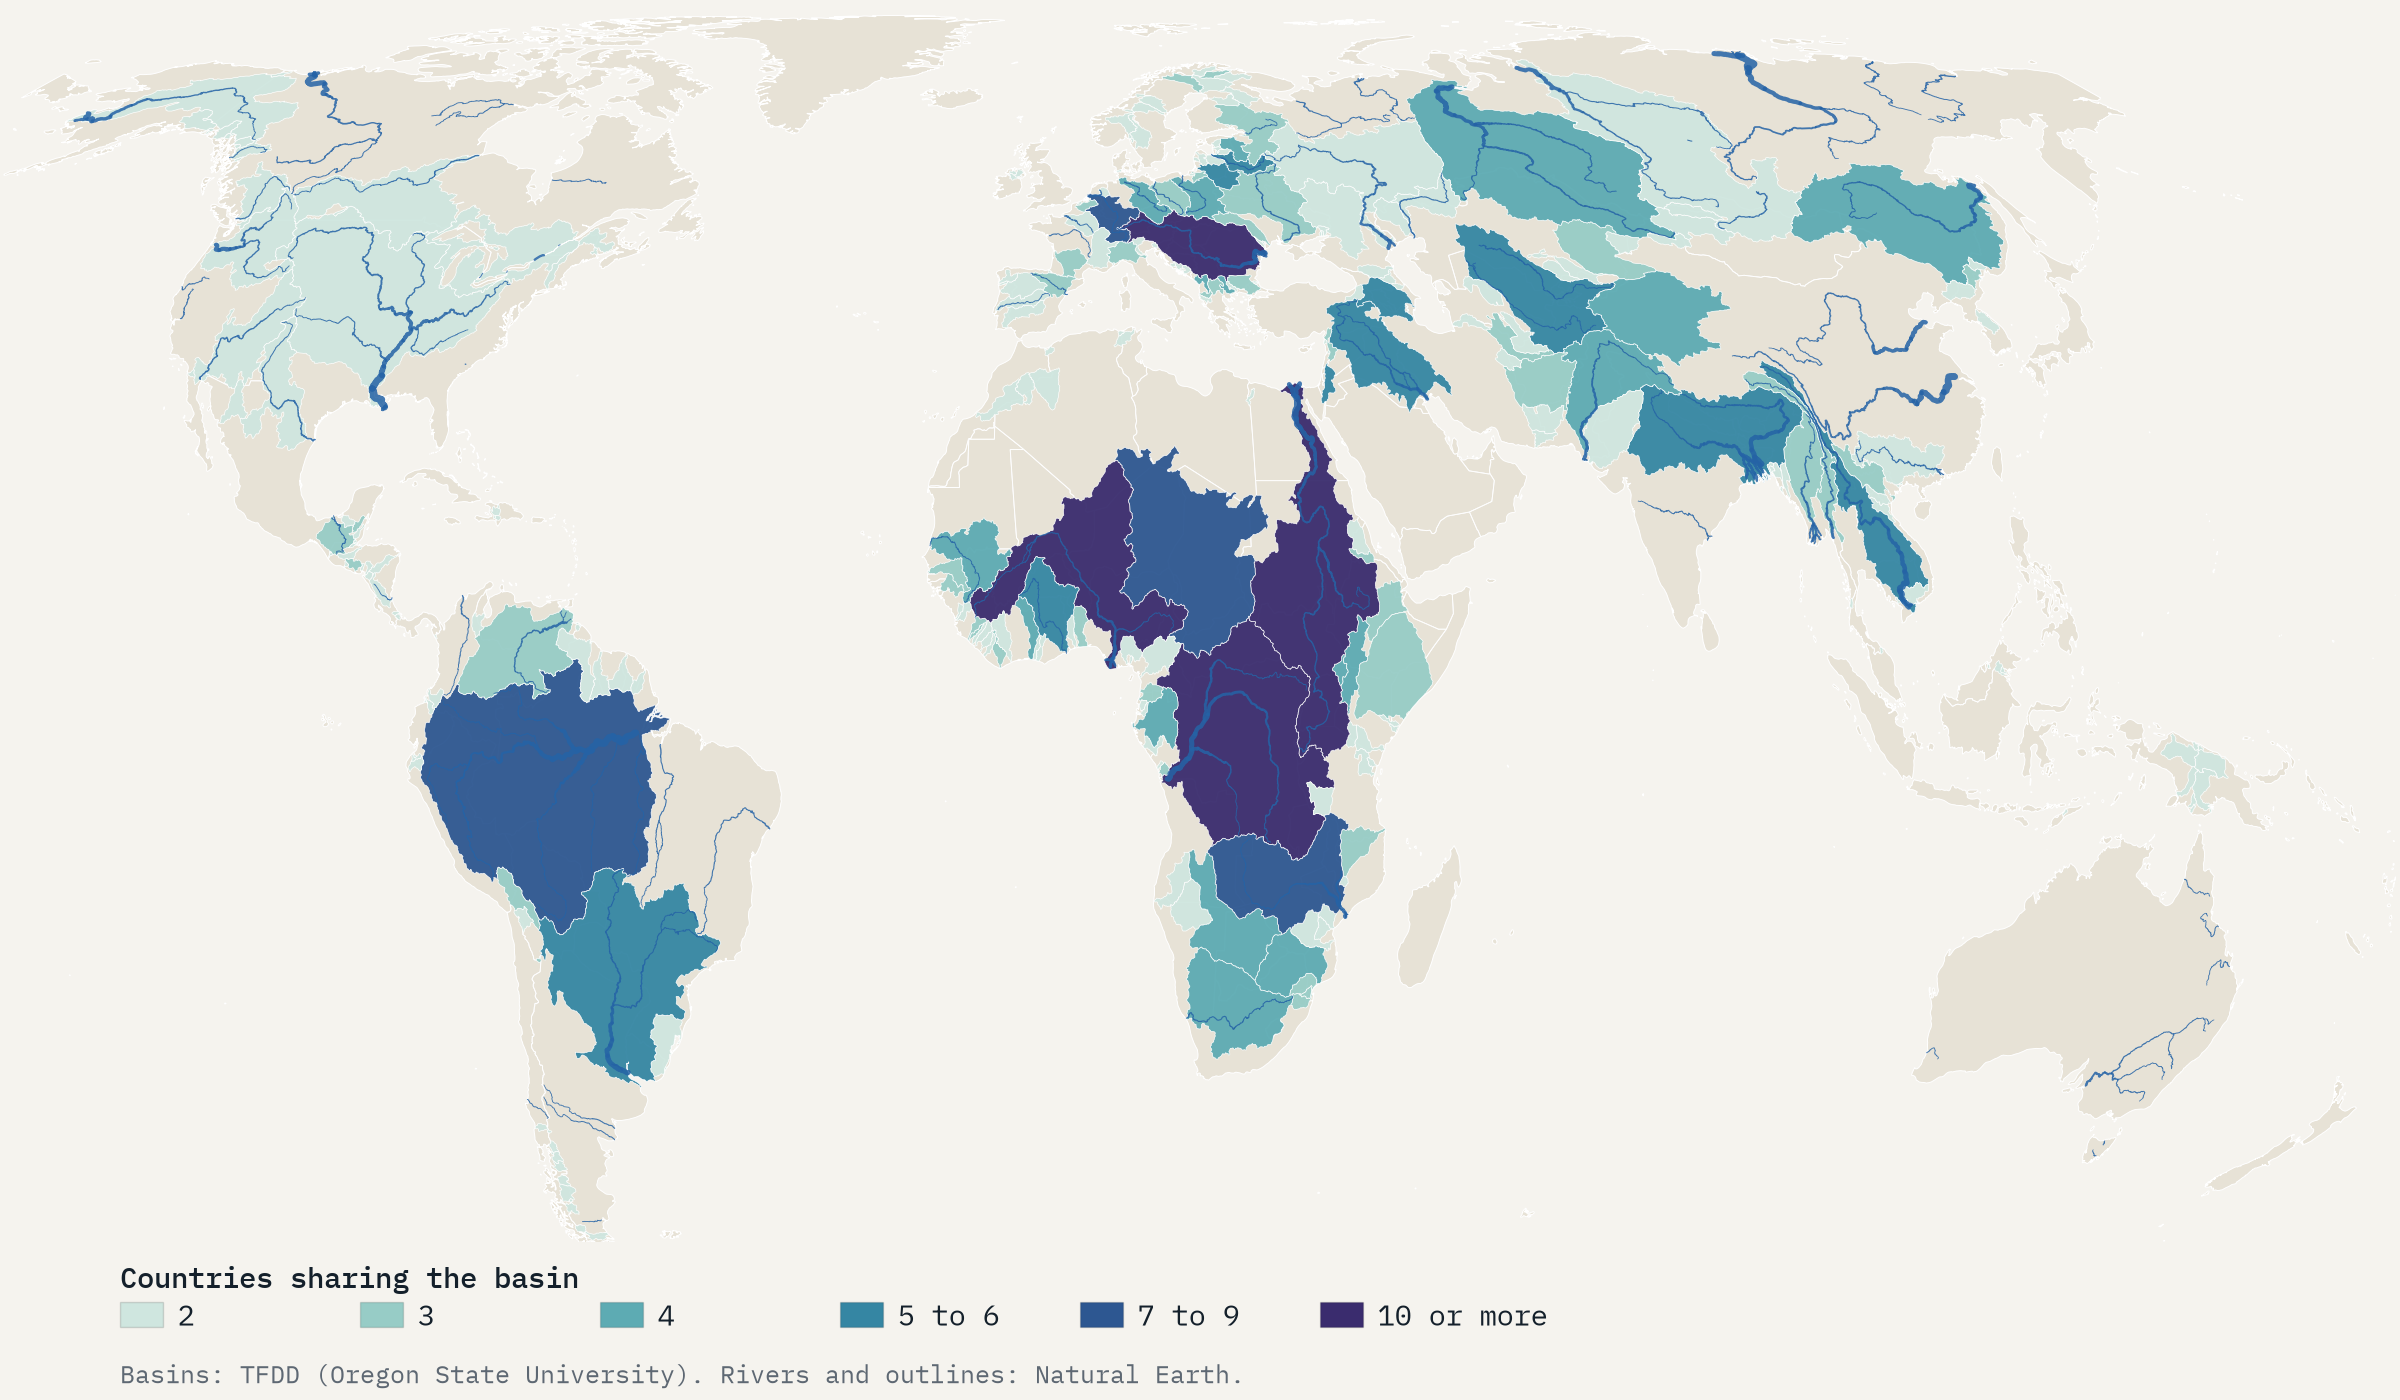
\includegraphics[width=\textwidth]{f_world_basins.png}
\caption{International river basins coloured by the number of countries sharing them (TFDD), with Natural Earth rivers.}\label{fig:world}\end{figure}

\begin{figure}[tbp]\centering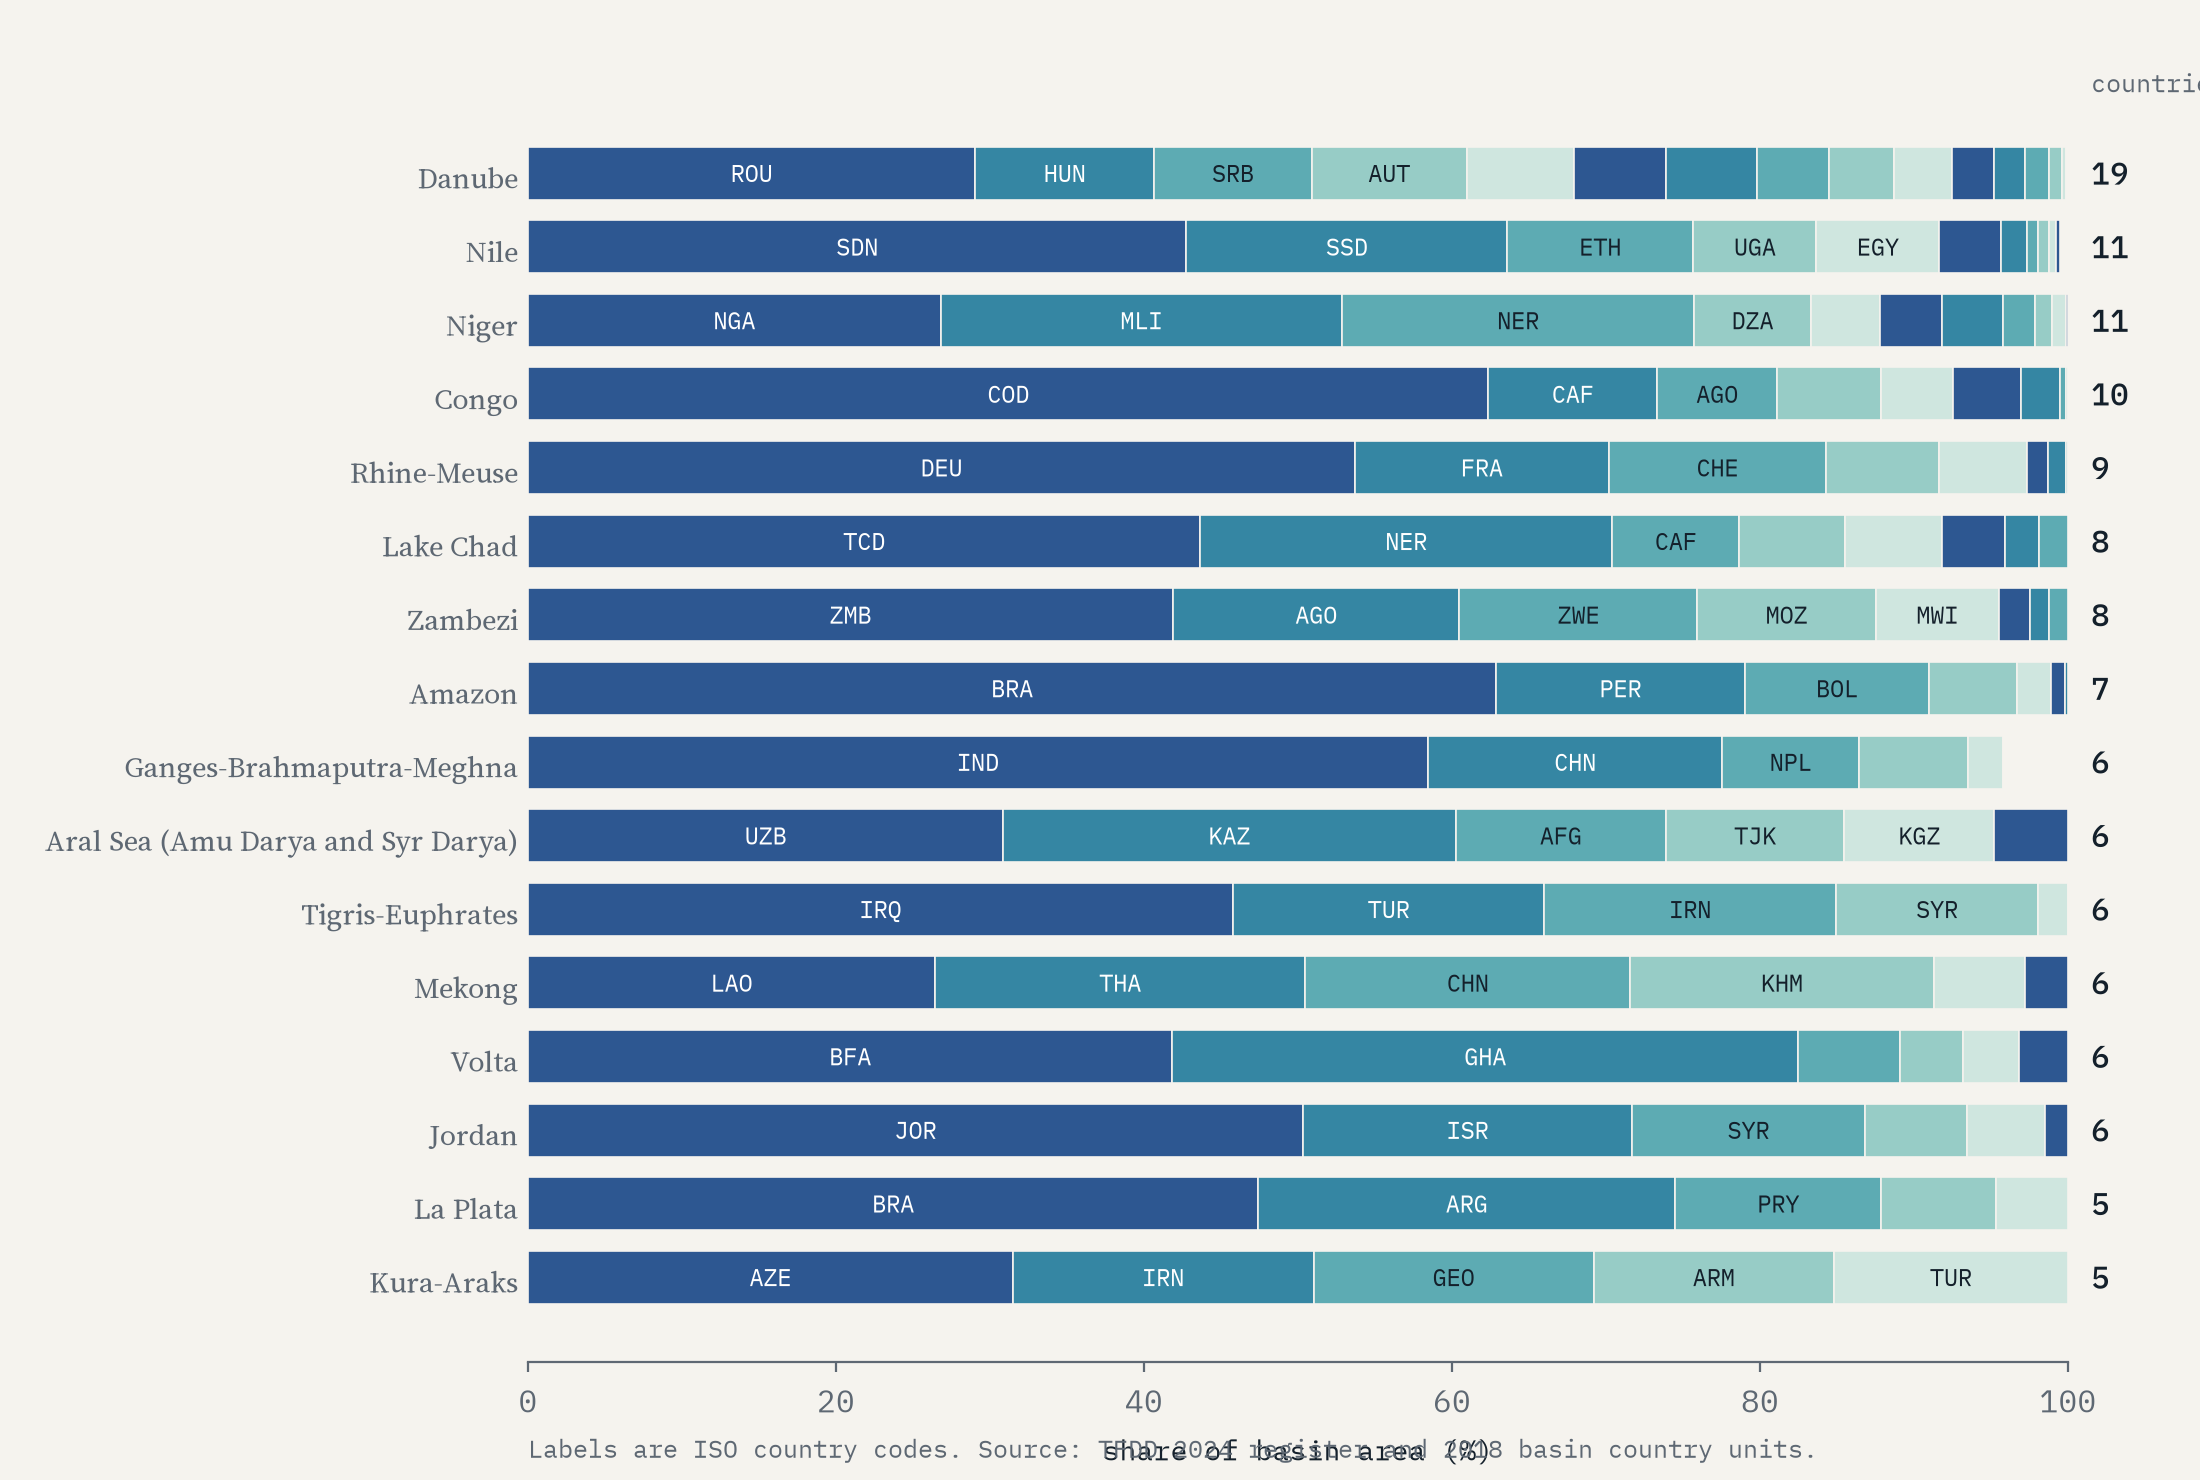
\includegraphics[width=.92\textwidth]{f_share_bars.png}
\caption{The basins shared by most countries, split by each country's share of basin area.}\label{fig:share}\end{figure}

\begin{table}[tbp]\centering\small\caption{The international basins shared by most countries. Area and population (2022) from the TFDD; largest shares from the basin country units.}\label{tab:top}\begin{tabular}{>{\raggedright\arraybackslash}p{3.6cm}rrr>{\raggedright\arraybackslash}p{5.4cm}}\toprule Basin & Countries & Area km\textsuperscript{2} & People (m) & Largest shares\\\midrule
Danube & 19 & 800,970 & 76.8 & Romania 29\%, Hungary 12\%, Serbia 10\%\\
Nile & 11 & 2,961,325 & 290.8 & Sudan 43\%, South Sudan 21\%, Ethiopia 12\%\\
Niger & 11 & 2,132,247 & 153.4 & Nigeria 27\%, Mali 26\%, Niger 23\%\\
Congo & 10 & 3,688,888 & 127.9 & DR Congo 62\%, Central African Republic 11\%, Angola 8\%\\
Rhine-Meuse & 9 & 198,295 & 61.9 & Germany 54\%, France 17\%, Switzerland 14\%\\
Lake Chad & 8 & 2,596,866 & 67.0 & Chad 44\%, Niger 27\%, Central African Republic 8\%\\
Zambezi & 8 & 1,374,975 & 53.6 & Zambia 42\%, Angola 19\%, Zimbabwe 15\%\\
Amazon & 7 & 5,952,595 & 35.8 & Brazil 63\%, Peru 16\%, Bolivia 12\%\\
Ganges-Brahmaputra-Meghna & 6 & 1,661,973 & 849.3 & India 58\%, China 19\%, Nepal 9\%\\
Aral Sea (Amu Darya and Syr Darya) & 6 & 1,218,379 & 63.4 & Uzbekistan 31\%, Kazakhstan 29\%, Afghanistan 14\%\\
Tigris-Euphrates & 6 & 868,989 & 79.2 & Iraq 46\%, Turkey 20\%, Iran 19\%\\
Mekong & 6 & 781,643 & 63.2 & Laos 26\%, Thailand 24\%, China 21\%\\
Volta & 6 & 411,243 & 33.4 & Burkina Faso 42\%, Ghana 41\%, Togo 7\%\\
Jordan & 6 & 45,005 & 13.5 & Jordan 50\%, Israel 21\%, Syria 15\%\\
La Plata & 5 & 2,981,517 & 116.9 & Brazil 47\%, Argentina 27\%, Paraguay 13\%\\
Kura-Araks & 5 & 189,893 & 14.3 & Azerbaijan 31\%, Iran 20\%, Georgia 18\%\\
\bottomrule\end{tabular}\end{table}

The most populous shared basin is the Ganges, Brahmaputra and Meghna, with 849 million people, more than the next two, the Nile (291 million) and the Indus (245 million), together (Figure~\ref{fig:pop}). 148 countries share at least one basin, and 32 have at least 99\% of their land in shared basins (Figure~\ref{fig:sharemap}). Russia shares the most basins (33), then United States (25) and Chile (21), many of them short rivers that cross long borders.

\begin{figure}[tbp]\centering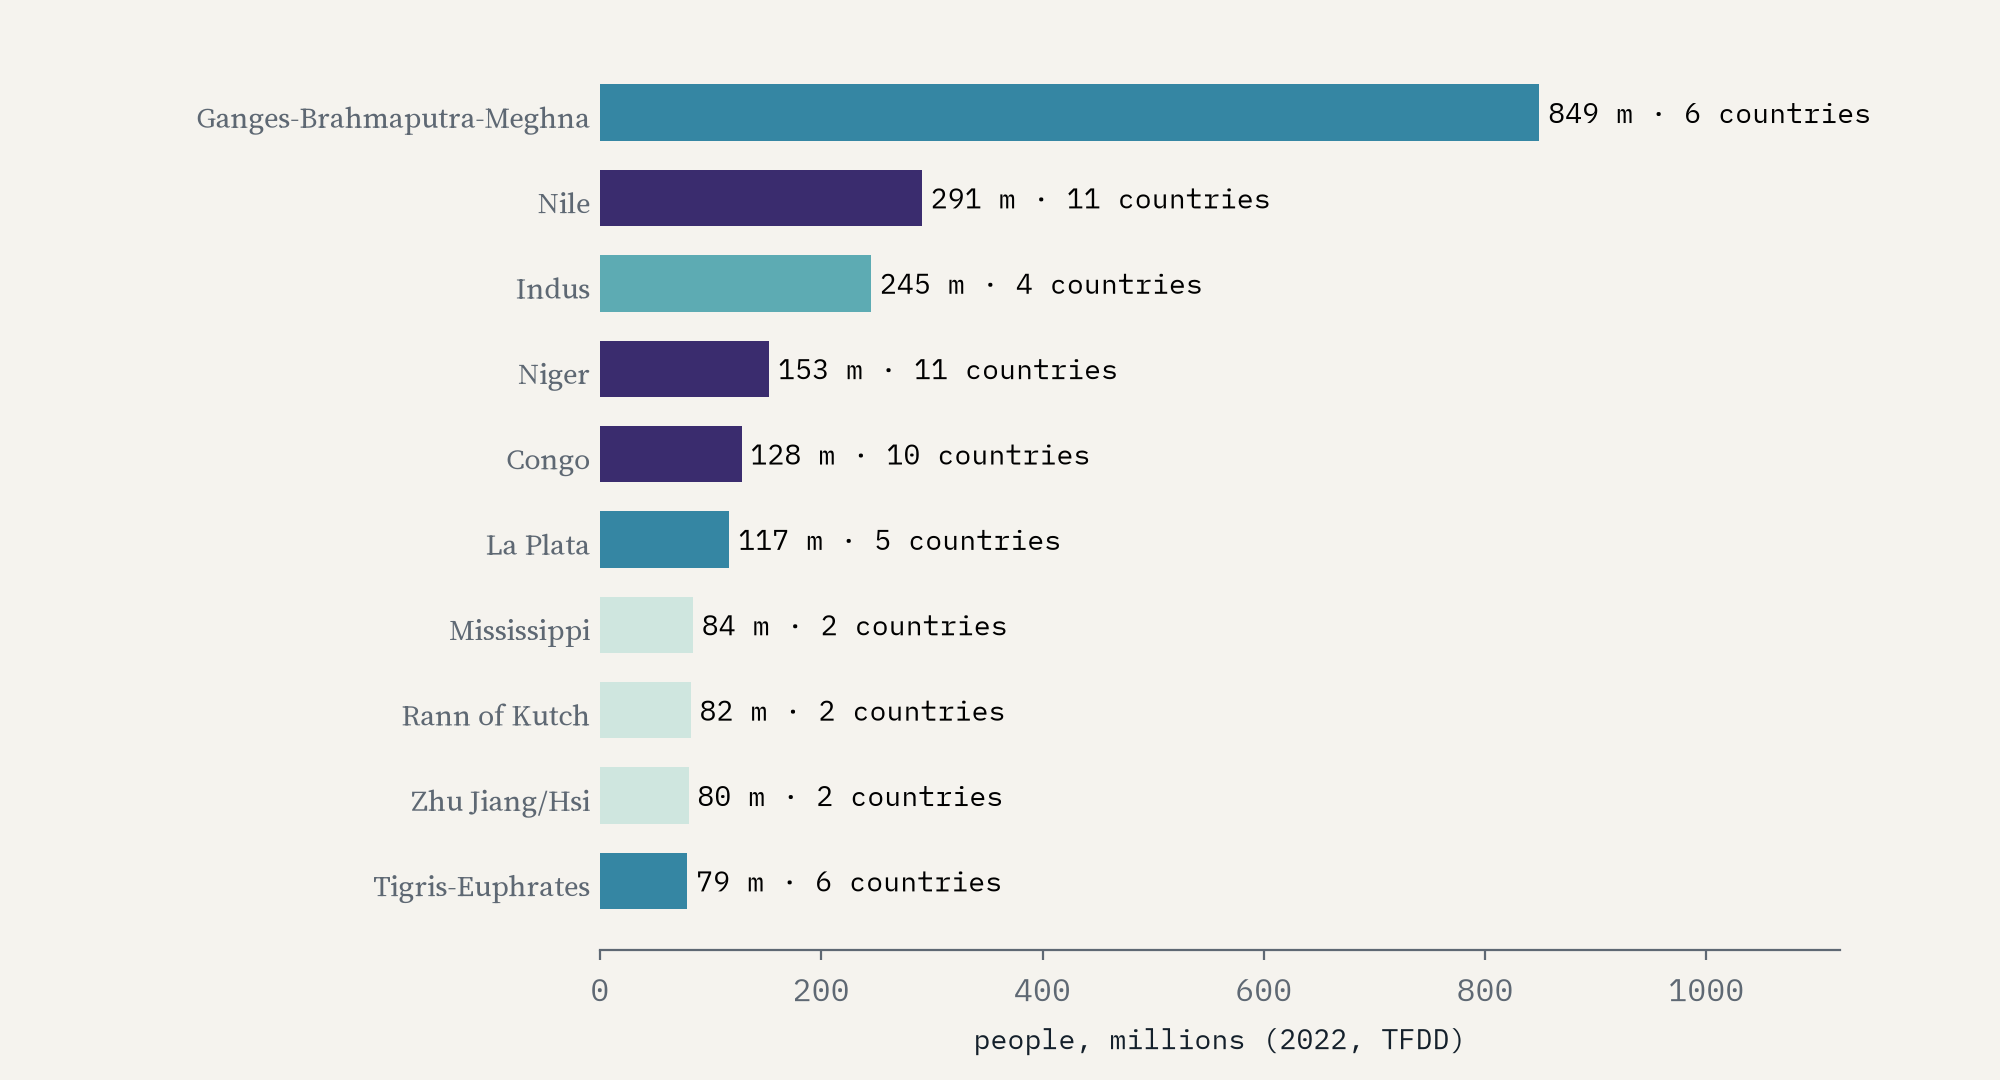
\includegraphics[width=.86\textwidth]{f_population.png}
\caption{The ten most populous international basins, 2022 (TFDD estimates), coloured by the number of countries sharing them.}\label{fig:pop}\end{figure}

\begin{figure}[tbp]\centering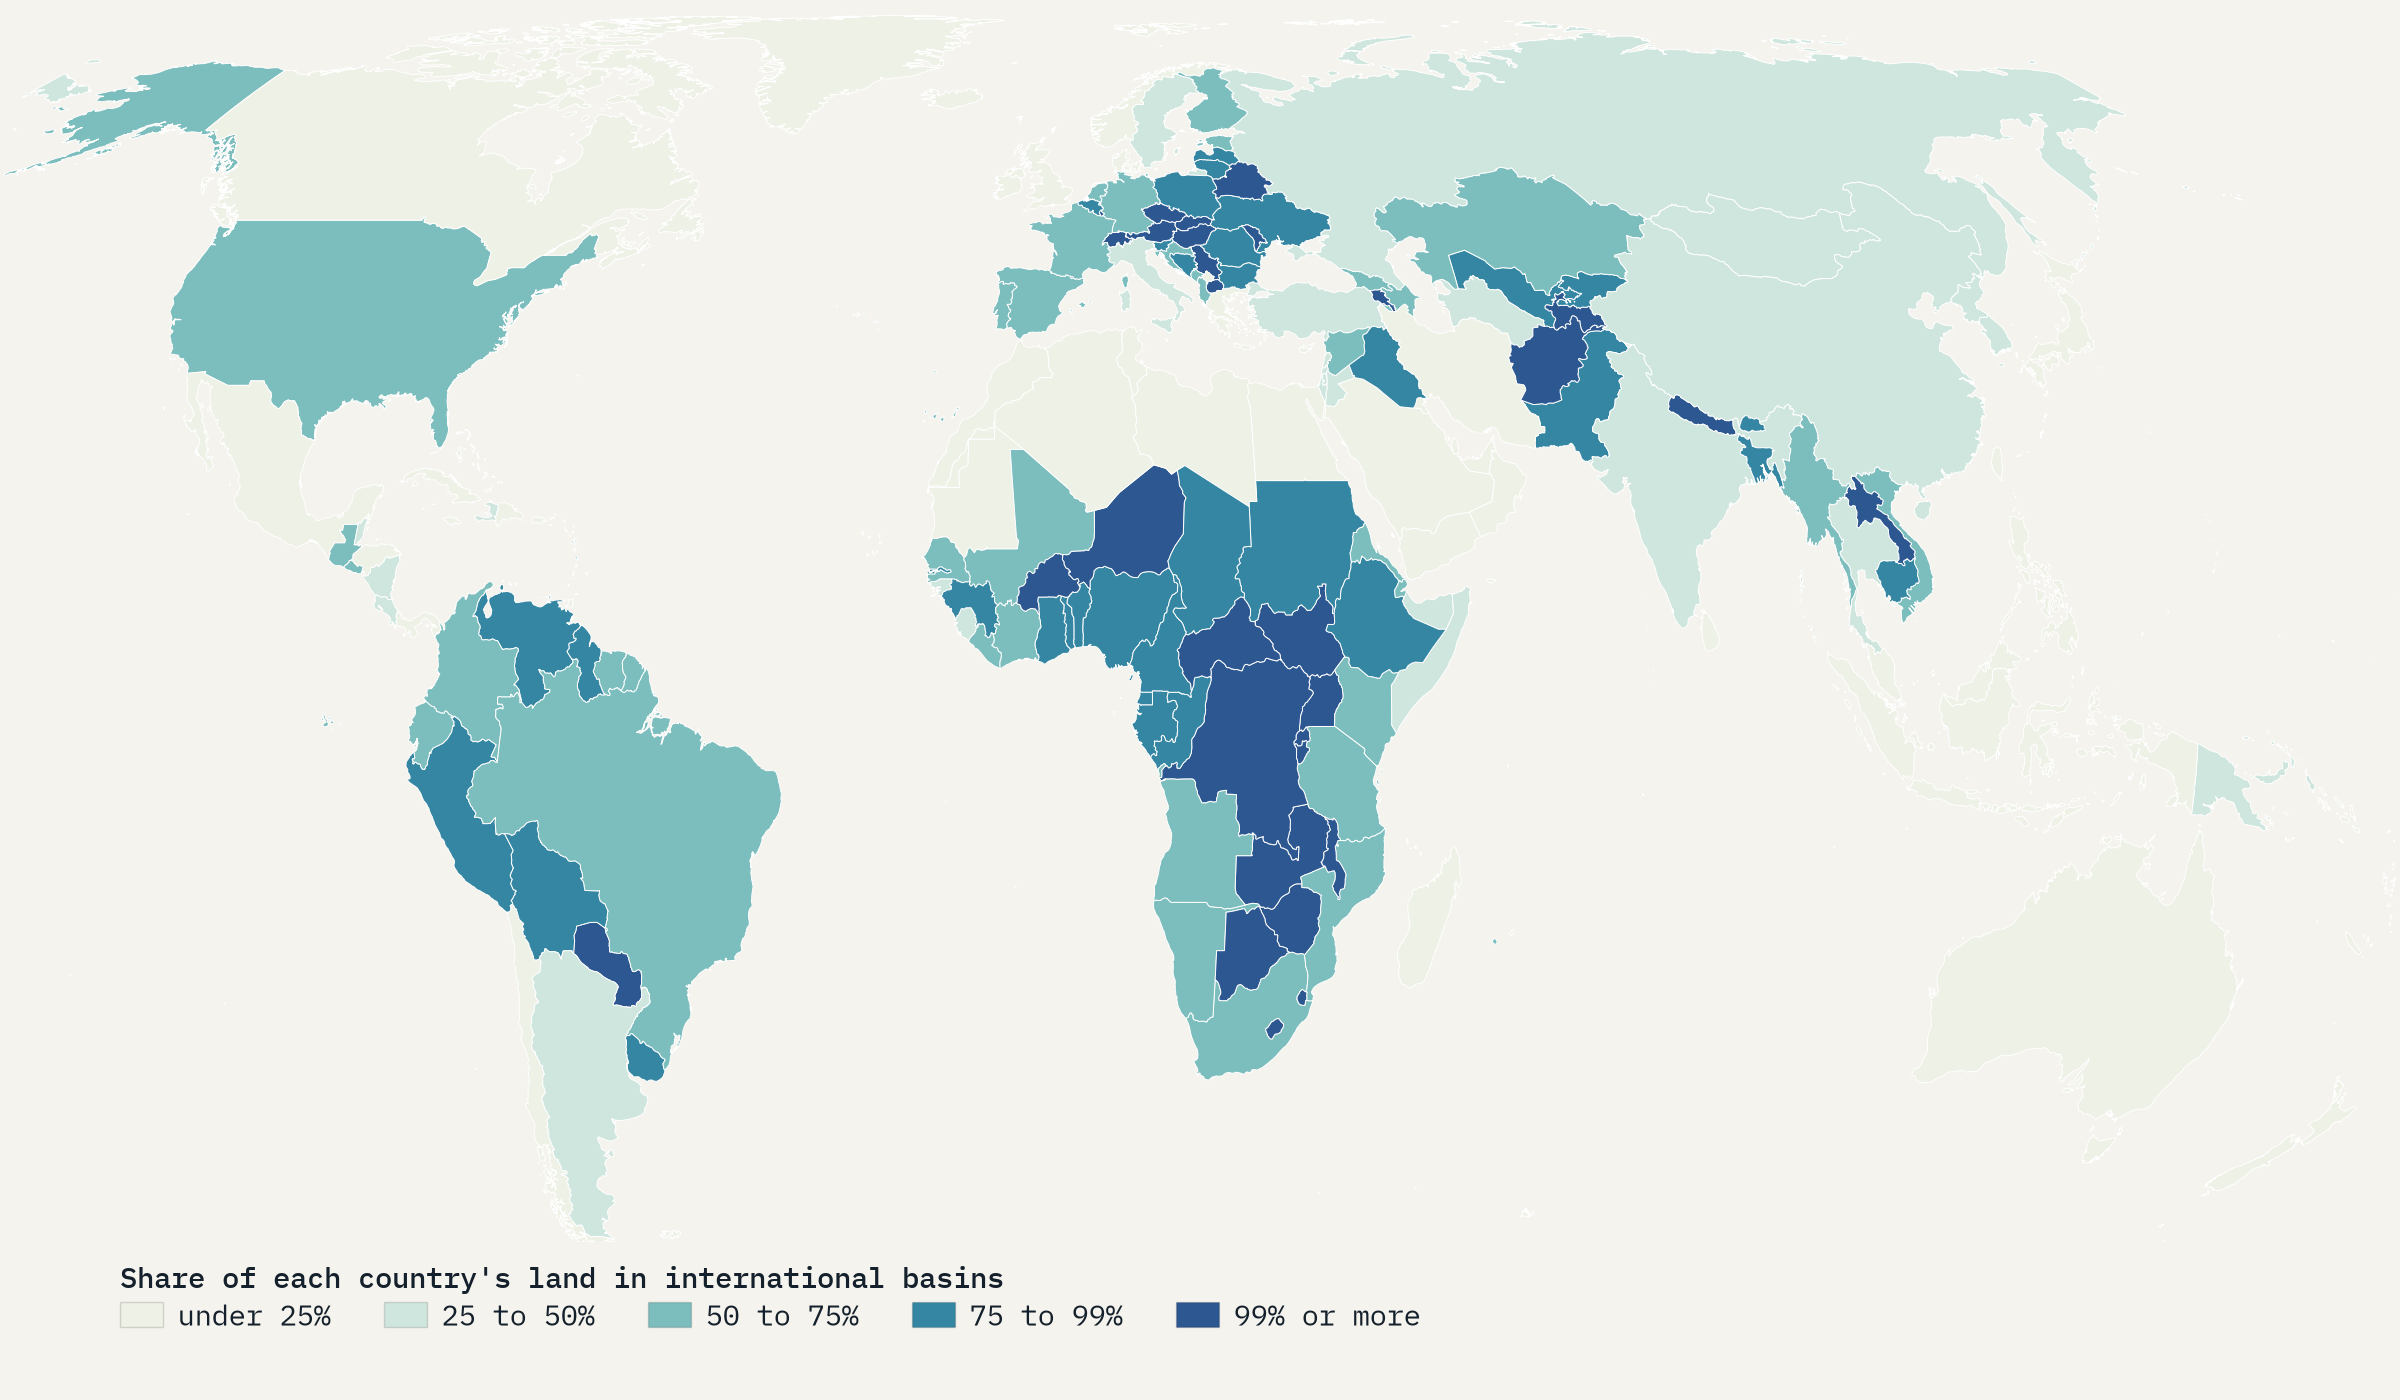
\includegraphics[width=\textwidth]{f_share_map.png}
\caption{Share of each country's land in international basins.}\label{fig:sharemap}\end{figure}

\begin{figure}[tbp]\centering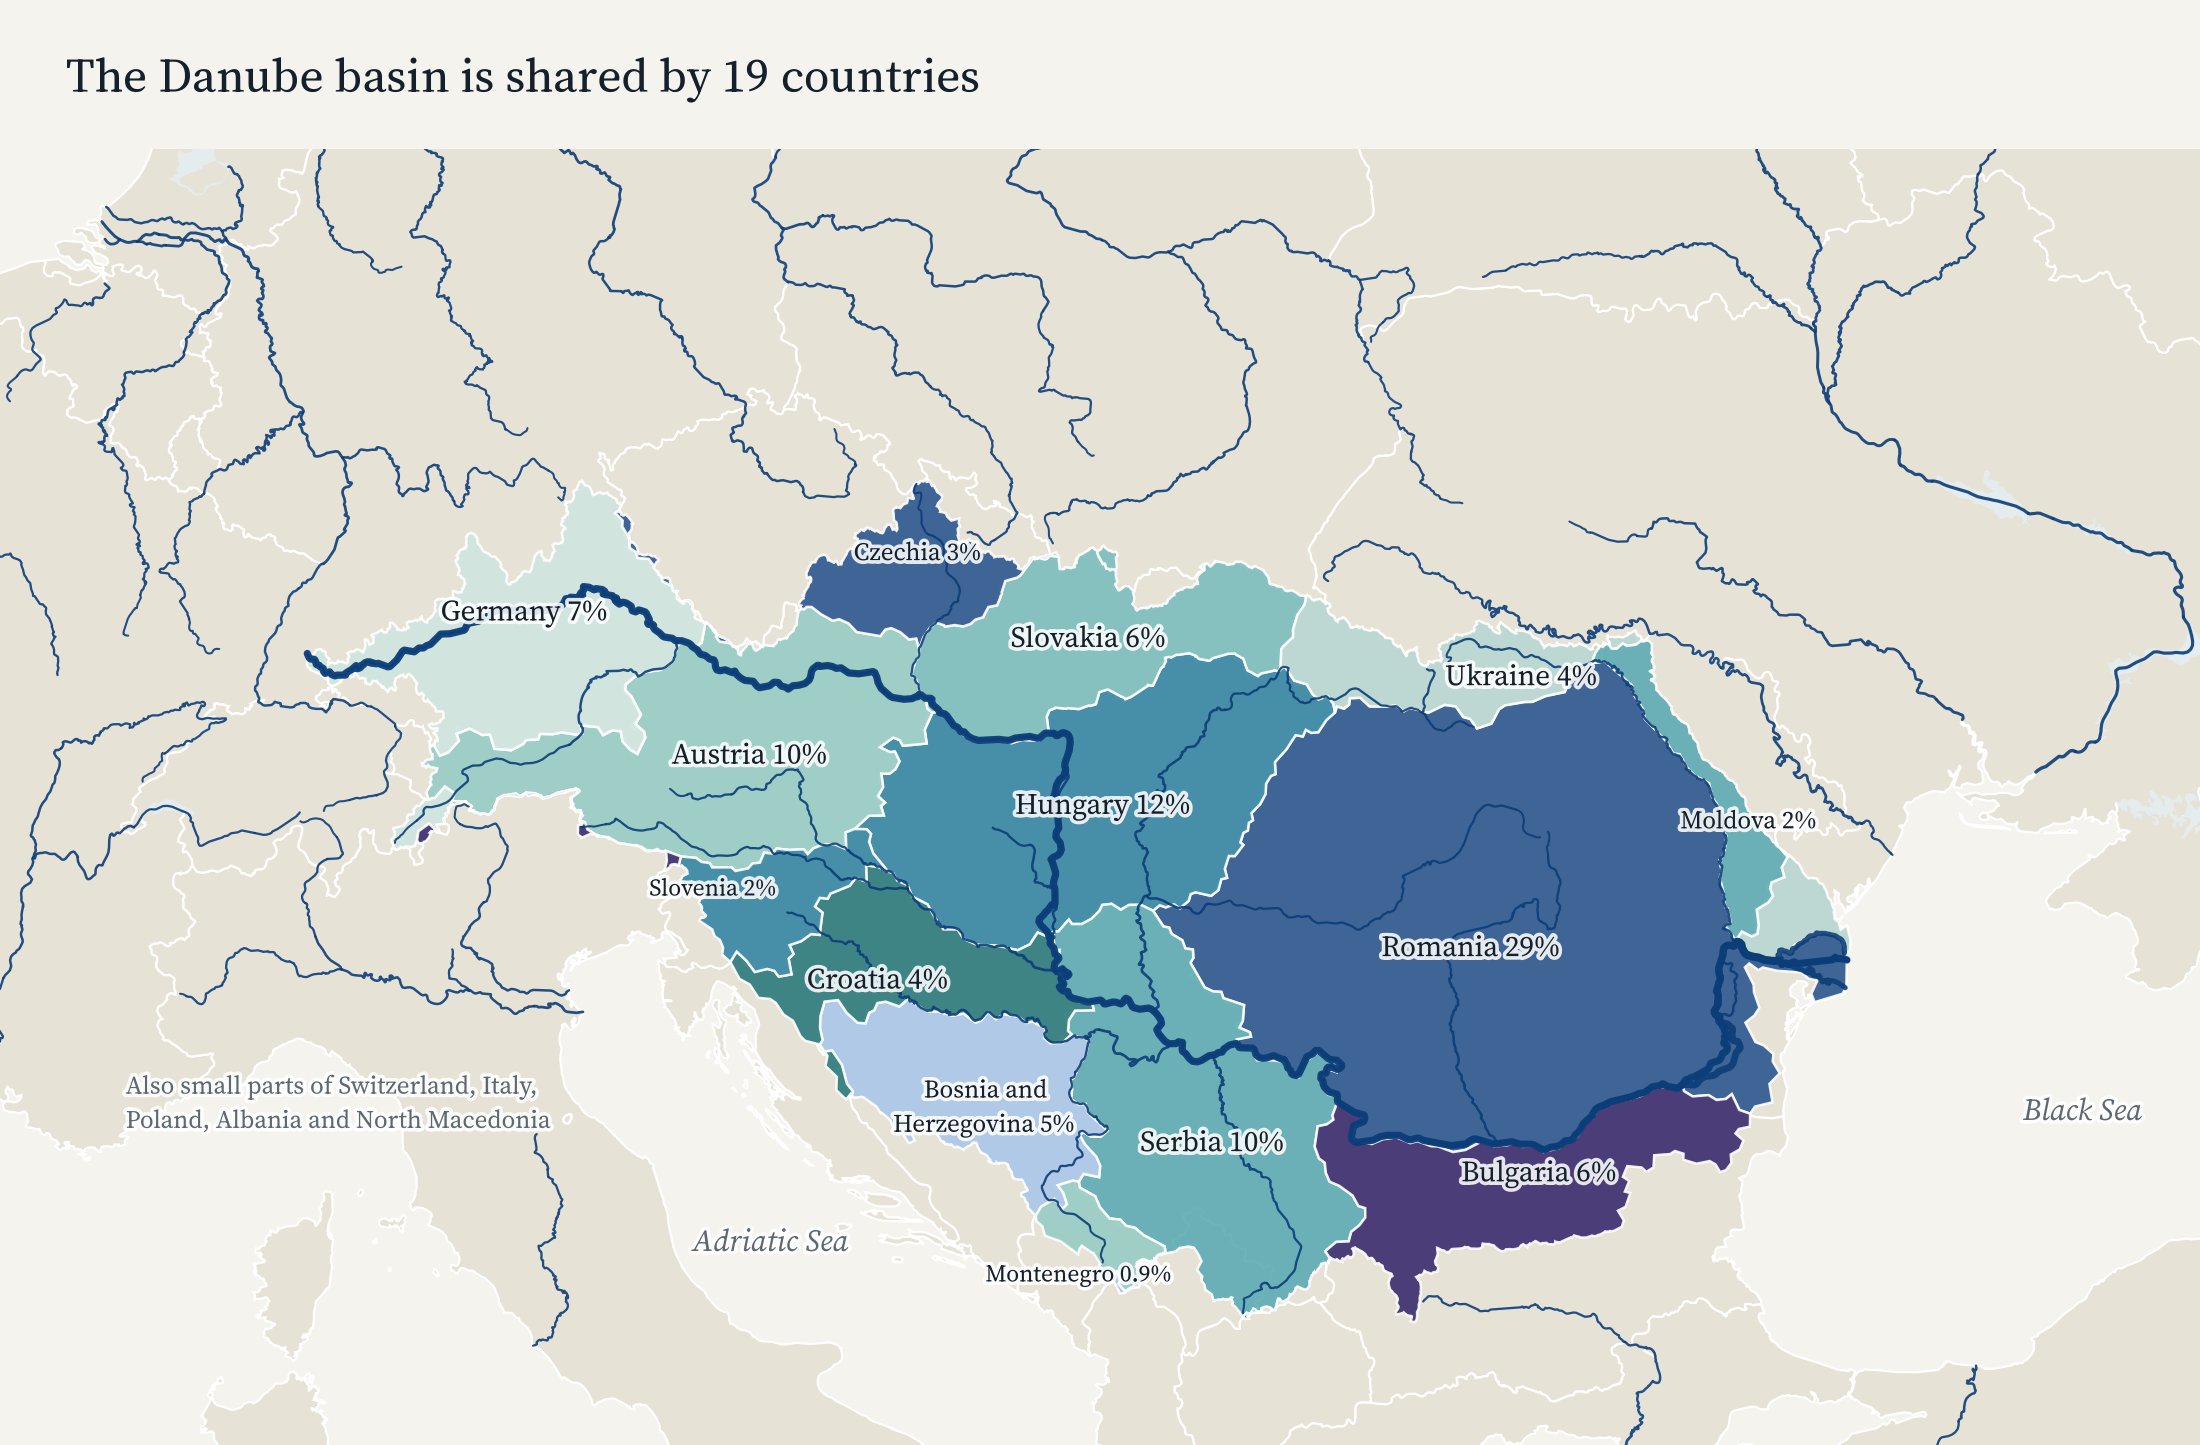
\includegraphics[width=.88\textwidth]{f_danube.png}
\caption{The Danube basin divided among its countries (TFDD basin country units), with the Natural Earth rivers and the longest path from the delta to the source (dark line).}\label{fig:danube}\end{figure}

\subsection{The longest rivers on one map}
Measured on the 1:10m lines, the longest systems are the Nile (6,151 km), the Yangtze (5,320 km), the Amazon (5,230 km), the Mississippi-Missouri (5,125 km) and the Yenisei-Angara (4,910 km) (Figure~\ref{fig:lengths}, Table~\ref{tab:rivers}). Of the ten longest, 7 drain international basins. All are shorter than published lengths. The Nile's map length is 92.5\% of Britannica's 6,650 km, the Amazon's 81.7\% of 6,400 km and the Yangtze's 84.4\% of 6,300 km \citep{brit_nile,brit_amazon,brit_yangtze}.

Three choices explain the gap. The first is scale. A line drawn for a 1:10 million map has lost its smaller bends, and the loss continues on coarser lines: on the 1:50m lines the Nile measures 5,682 km (92.4\% of its 1:10m length) and the Yangtze 4,699 km. Simplifying the 1:10m paths shortens them steadily, by 16\% for the Nile and 24\% for the Amazon at a tolerance of 0.5 degrees, with no sign of settling (Figure~\ref{fig:scale}). This is the coastline effect \citep{mandelbrot1967}: a wiggly line has no single length, only a length at a given resolution. The second is the mouth. Natural Earth's land outline opens into the Amazon estuary at 52.7°W, so its Amazon reaches the sea well inside the estuary, and the long-running argument over whether the Amazon is longer than the Nile turns partly on whether its mouth is drawn through the Pará estuary. The third is the source. Natural Earth's Amazon follows the Ucayali to the Andes of southern Peru, at 15.3°S; its Nile follows the White Nile, Lake Victoria and the Kagera to a source in Burundi. Taking the Blue Nile's source instead gives 4,708 km on the same map (Figure~\ref{fig:nile}), and taking the Mississippi's own source rather than the Missouri's gives 3,181 km rather than 5,125.

\begin{figure}[tbp]\centering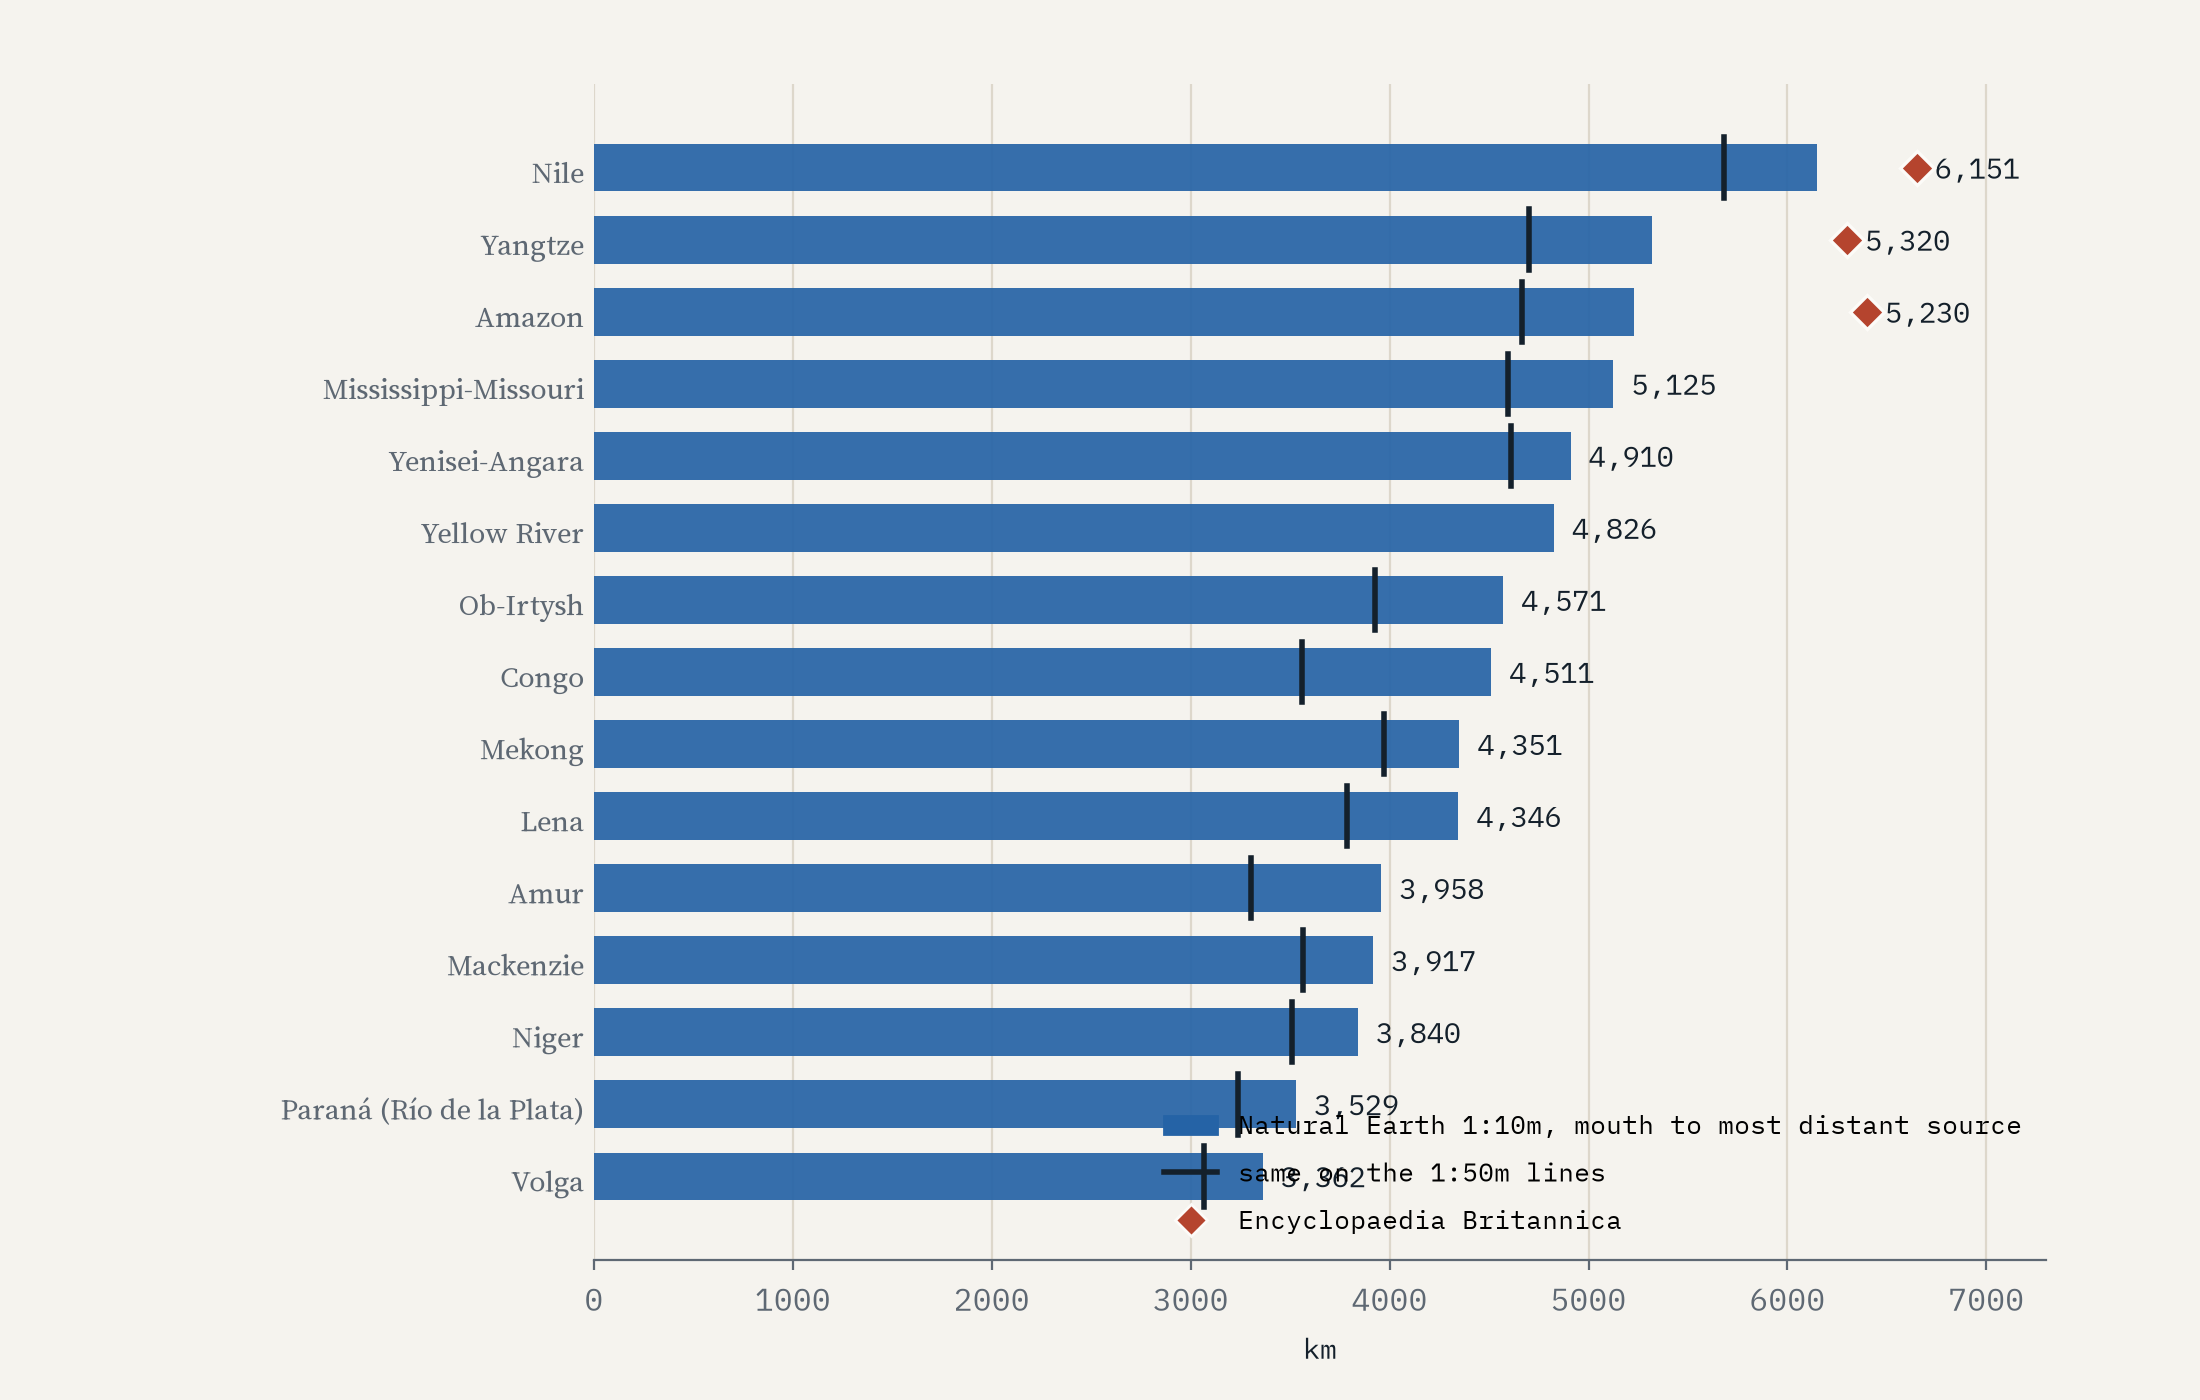
\includegraphics[width=.9\textwidth]{f_lengths.png}
\caption{The longest river systems: mouth to most distant source on the Natural Earth 1:10m lines (bars), the same on the 1:50m lines (ticks), and Britannica's lengths where quoted (diamonds).}\label{fig:lengths}\end{figure}

\begin{table}[tbp]\centering\small\caption{The longest river systems on the Natural Earth lines: mouth to most distant source (km), countries along that path, and the first rivers on the path from the mouth. n/a: no matching system on the 1:50m lines.}\label{tab:rivers}\setlength{\tabcolsep}{4pt}\begin{tabular}{rlrrr>{\raggedright\arraybackslash}p{6.2cm}}\toprule & System & 1:10m & 1:50m & Countries & Path from the mouth\\\midrule
1 & Nile & 6,151 & 5,682 & 7 & Rosetta Branch < Nile < El Bahr el Abyad < Bahr el  Zeraf\\
2 & Yangtze & 5,320 & 4,699 & 1 & Yangtze < Jinsha < Tongtian < Tuotuo\\
3 & Amazon & 5,230 & 4,664 & 3 & Amazon < Ucayali\\
4 & Mississippi-Missouri & 5,125 & 4,594 & 1 & Bayou Lafourche < Mississippi < Missouri < Madison\\
5 & Yenisei-Angara & 4,910 & 4,611 & 2 & Yenisei < Angara < Selenga < Ideriyn\\
6 & Yellow River & 4,826 & n/a & 1 & Yellow River\\
7 & Ob-Irtysh & 4,571 & 3,928 & 3 & Ob < Malaya Ob < Irtysh < Ertis\\
8 & Congo & 4,511 & 3,561 & 4 & Congo < Lualaba < Luvua < Luapula\\
9 & Mekong & 4,351 & 3,974 & 6 & Mekong < Lancang < Za\\
10 & Lena & 4,346 & 3,788 & 1 & Bykovskaya Protoka < Lena < Vitim\\
11 & Amur & 3,958 & 3,305 & 3 & Amur < Heilong Jiang < Shilka < Onon\\
12 & Mackenzie & 3,917 & 3,564 & 1 & Mackenzie < Slave < Peace < Finlay\\
13 & Niger & 3,840 & 3,509 & 5 & Niger\\
14 & Paraná (Río de la Plata) & 3,529 & 3,240 & 3 & Paraná < Grande\\
15 & Volga & 3,362 & 3,067 & 1 & Volga < Oka\\
\bottomrule\end{tabular}\end{table}

\begin{figure}[tbp]\centering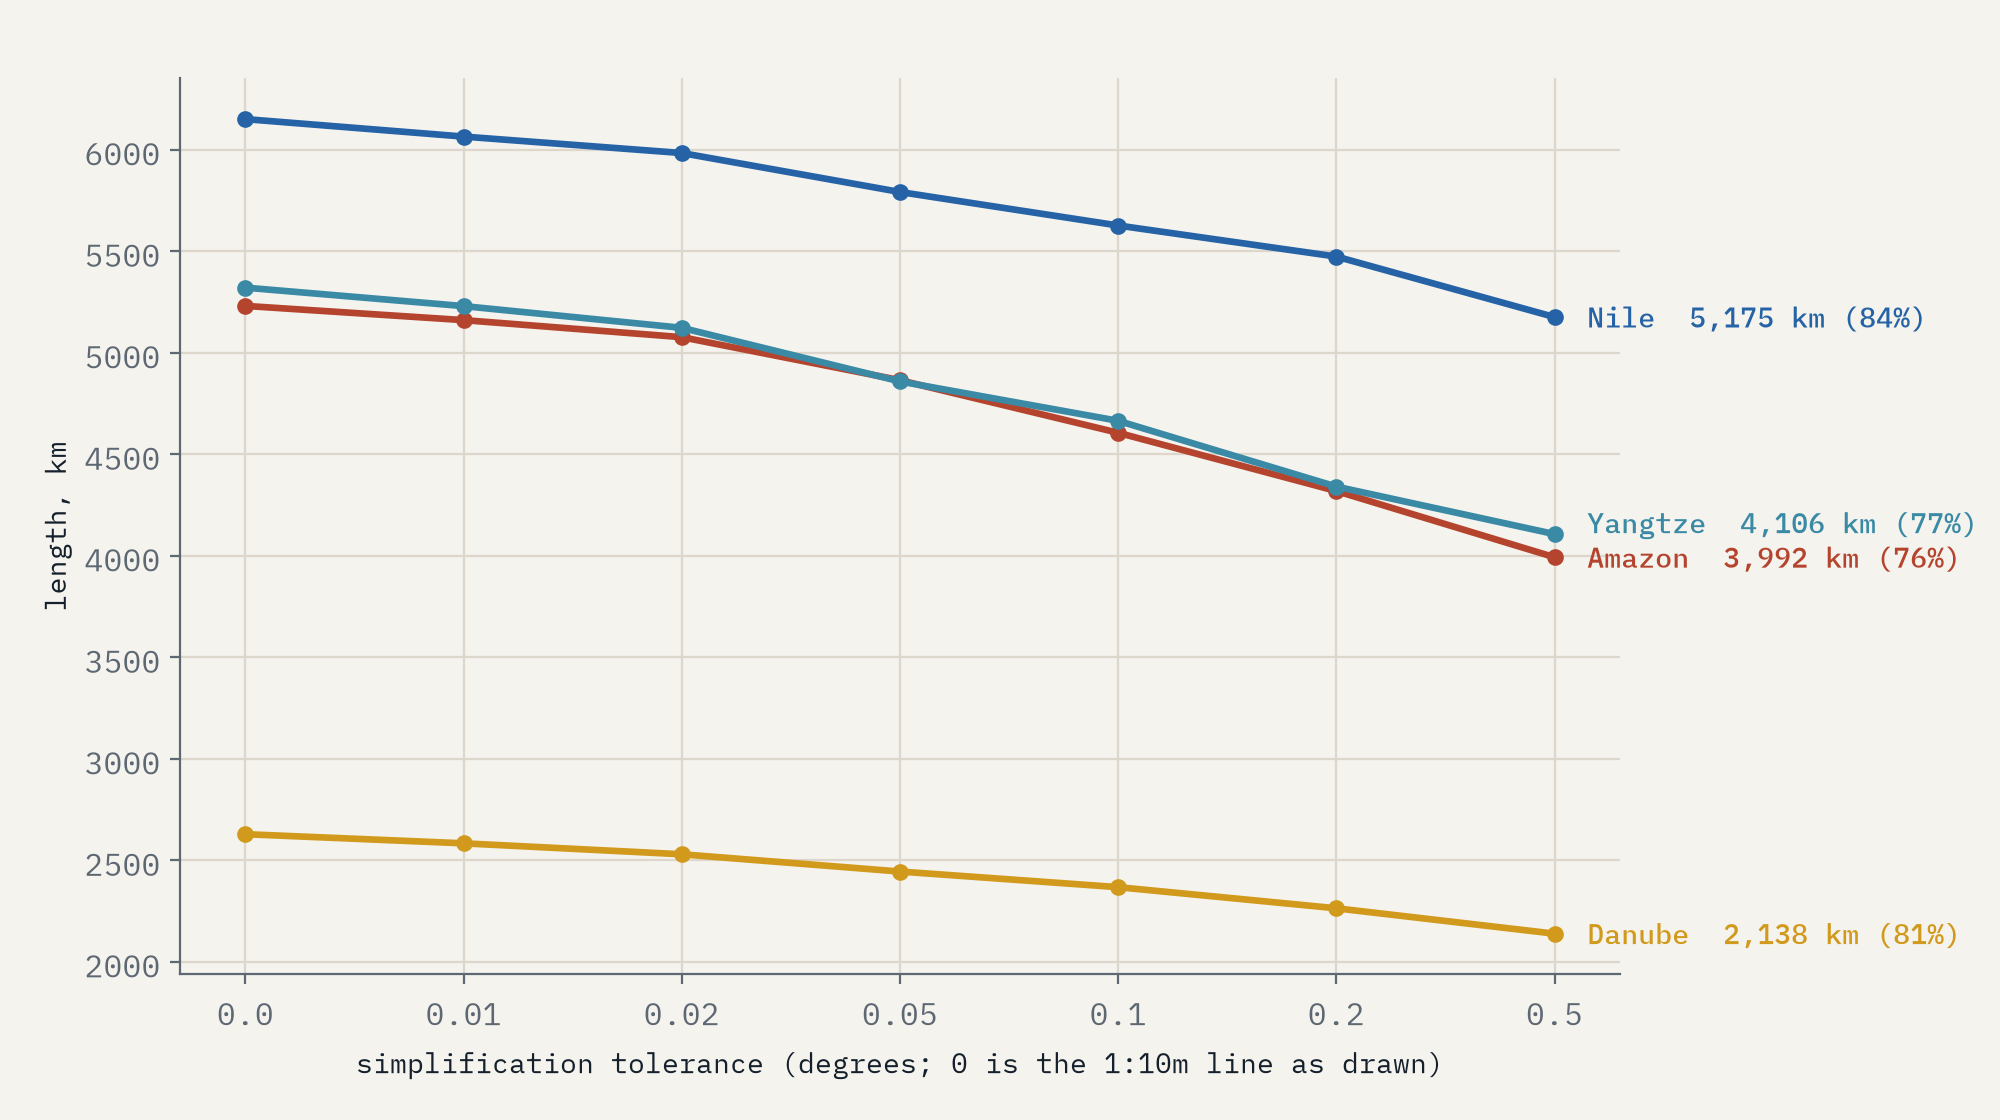
\includegraphics[width=.86\textwidth]{f_scale.png}
\caption{Length of four mouth-to-source paths as the 1:10m lines are simplified (Douglas and Peucker tolerance in degrees).}\label{fig:scale}\end{figure}

\begin{figure}[tbp]\centering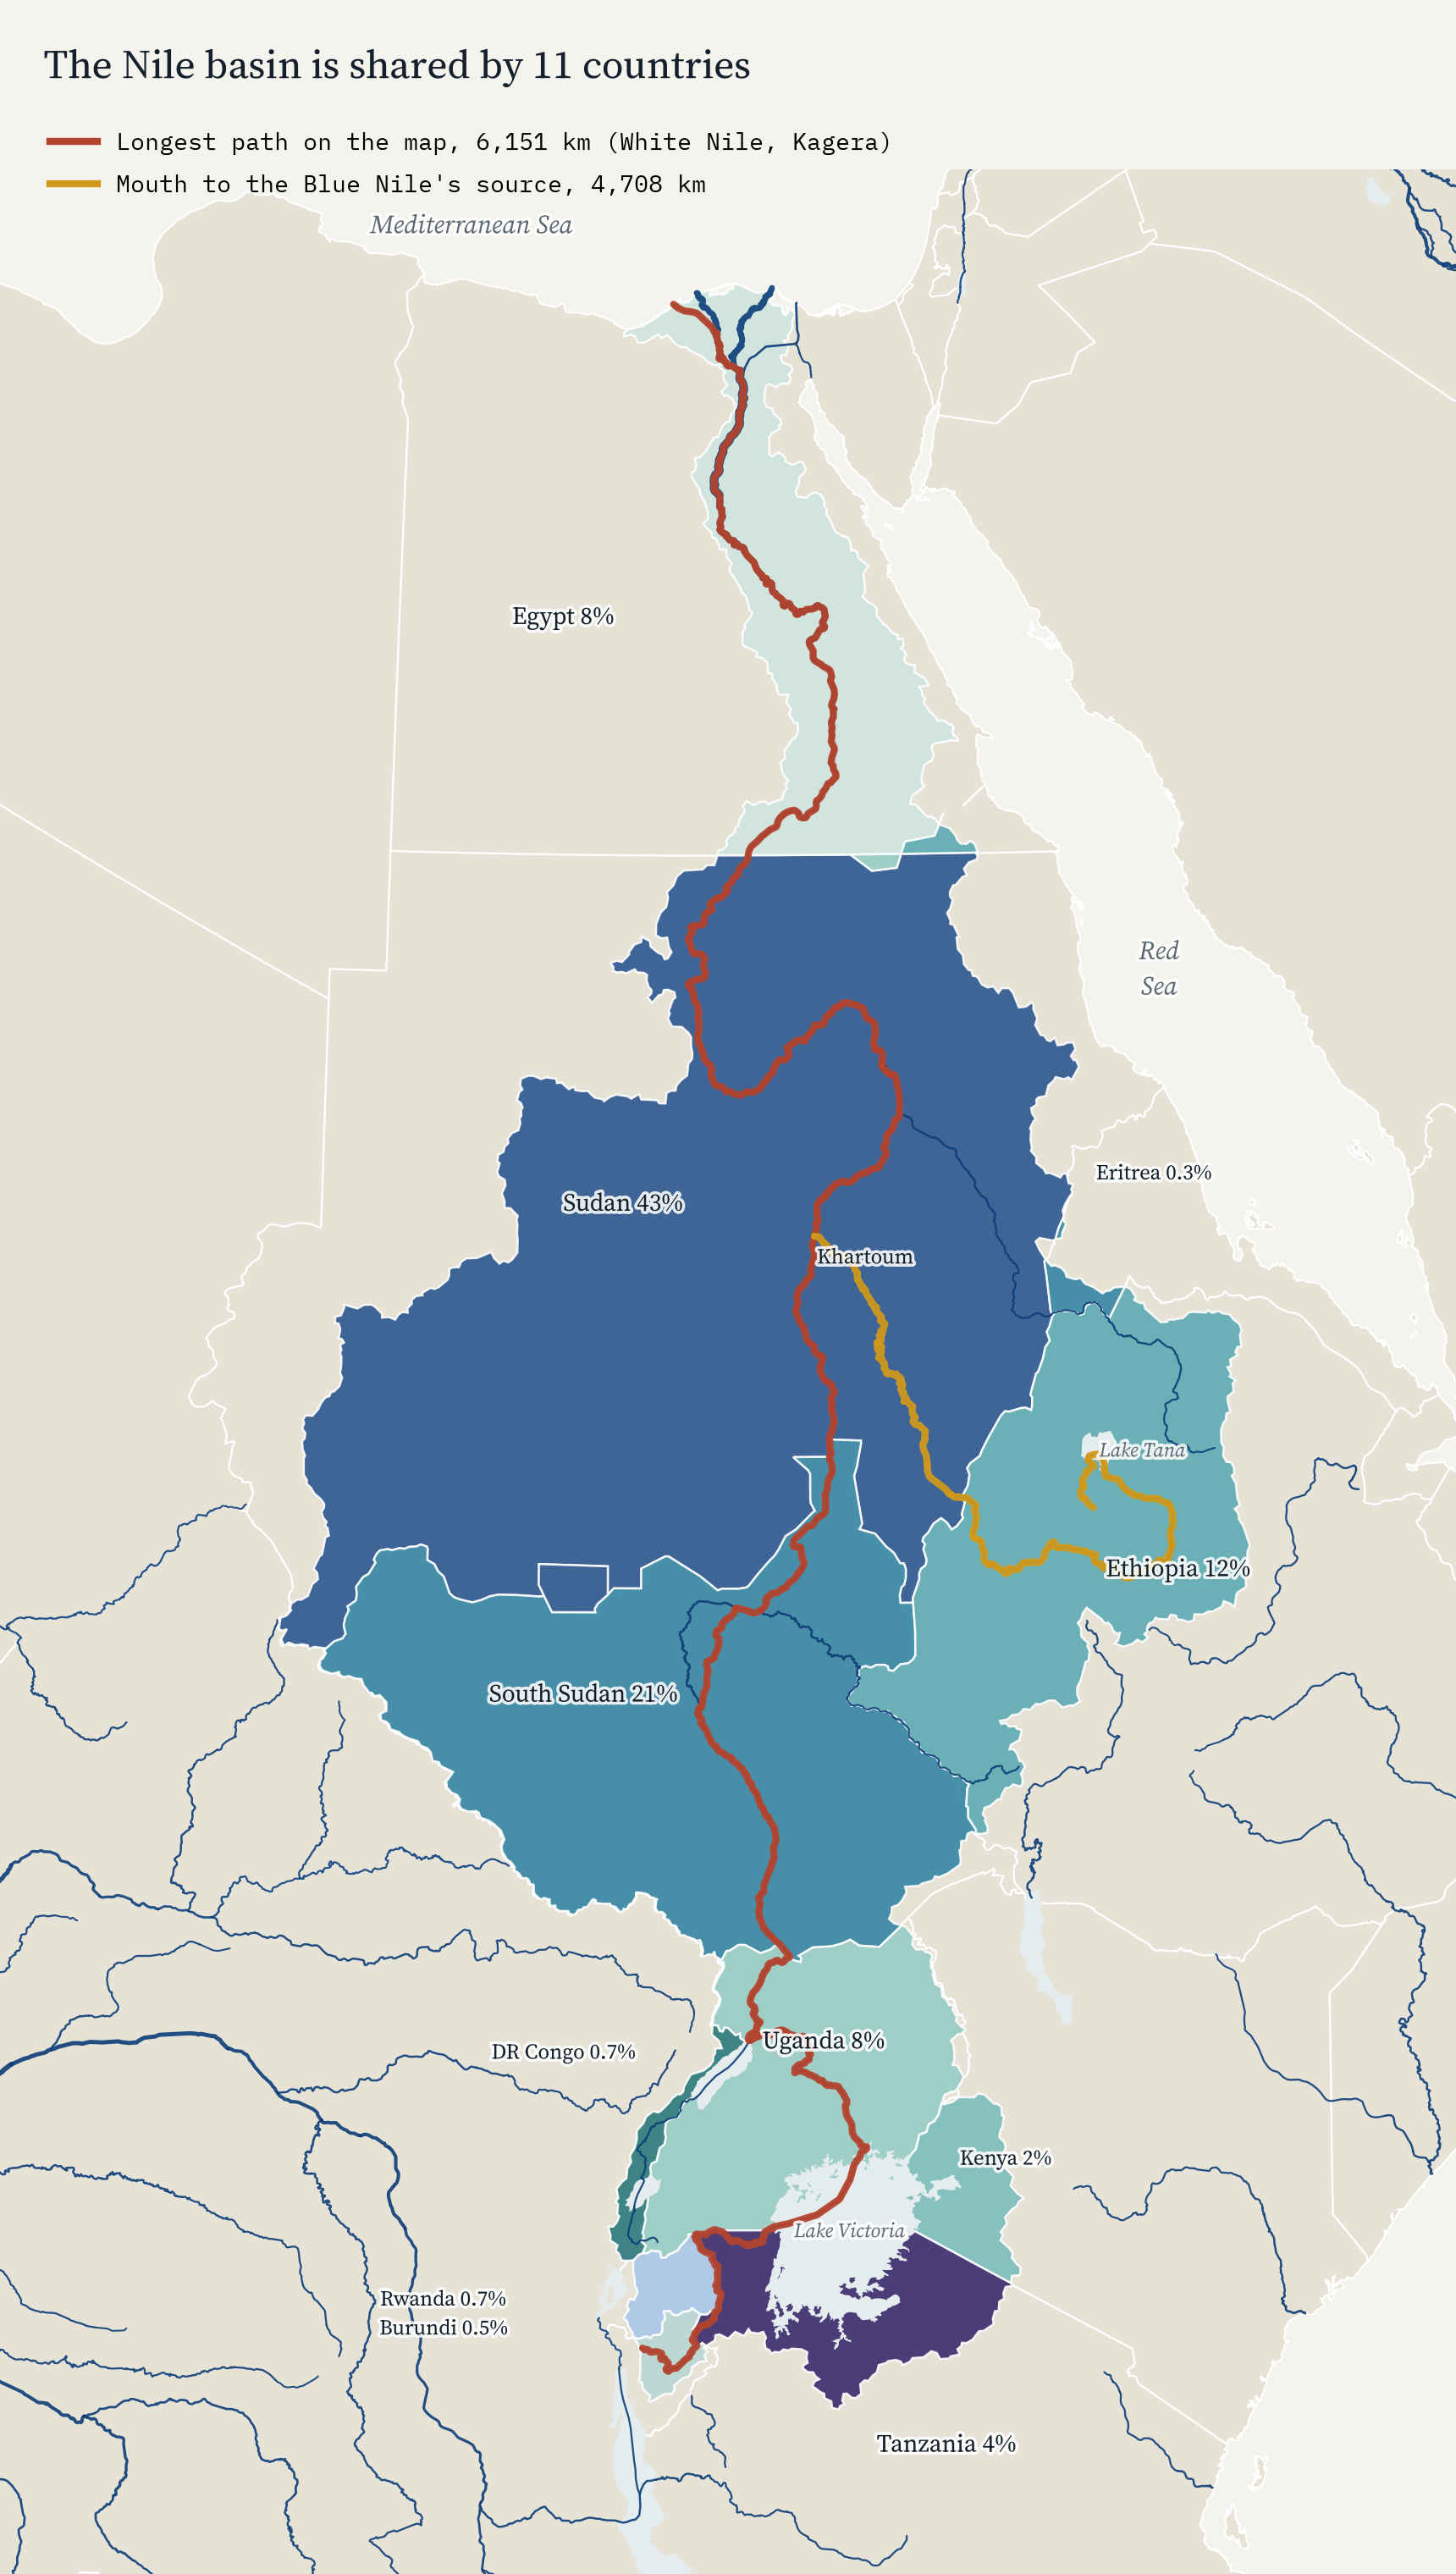
\includegraphics[width=.72\textwidth]{f_nile.png}
\caption{The Nile basin divided among its countries, with the longest path on the map (White Nile and Kagera) and the path to the Blue Nile's source.}\label{fig:nile}\end{figure}

\subsection{Rivers across borders}
Counting the countries a named river flows through or along, the Danube leads with 9, from Germany to Ukraine, followed by the Mekong and the Rhine with 6 each and the Niger and the Zambezi with 5. The usual count for the Danube is ten; the method misses Moldova, whose bank of the Danube is too short to register at this scale (Natural Earth's outline of Moldova stops 1.7 km from the river line). The longest path of the Nile system crosses or follows 7 countries, fewer than the 11 that share its basin.

\subsection{Water from abroad}
For 38 of 191 countries, more than half of the renewable water originates outside the country, and for 17 more than three quarters (Figures~\ref{fig:dep} and \ref{fig:depbars}). The highest ratios belong to Kuwait (100.0\%) and Bahrain (96.5\%), which have no rivers and whose small renewable supply is counted as groundwater from outside. Among river countries the list is led by Turkmenistan (97.0\%), Egypt (96.9\%), Mauritania (96.5\%) and Sudan (96.1\%), then Hungary (94.2\%), Bangladesh (91.4\%), Niger (89.7\%) and the Netherlands (87.9\%): deltas, dry lowlands and the lower ends of long rivers.

\begin{figure}[tbp]\centering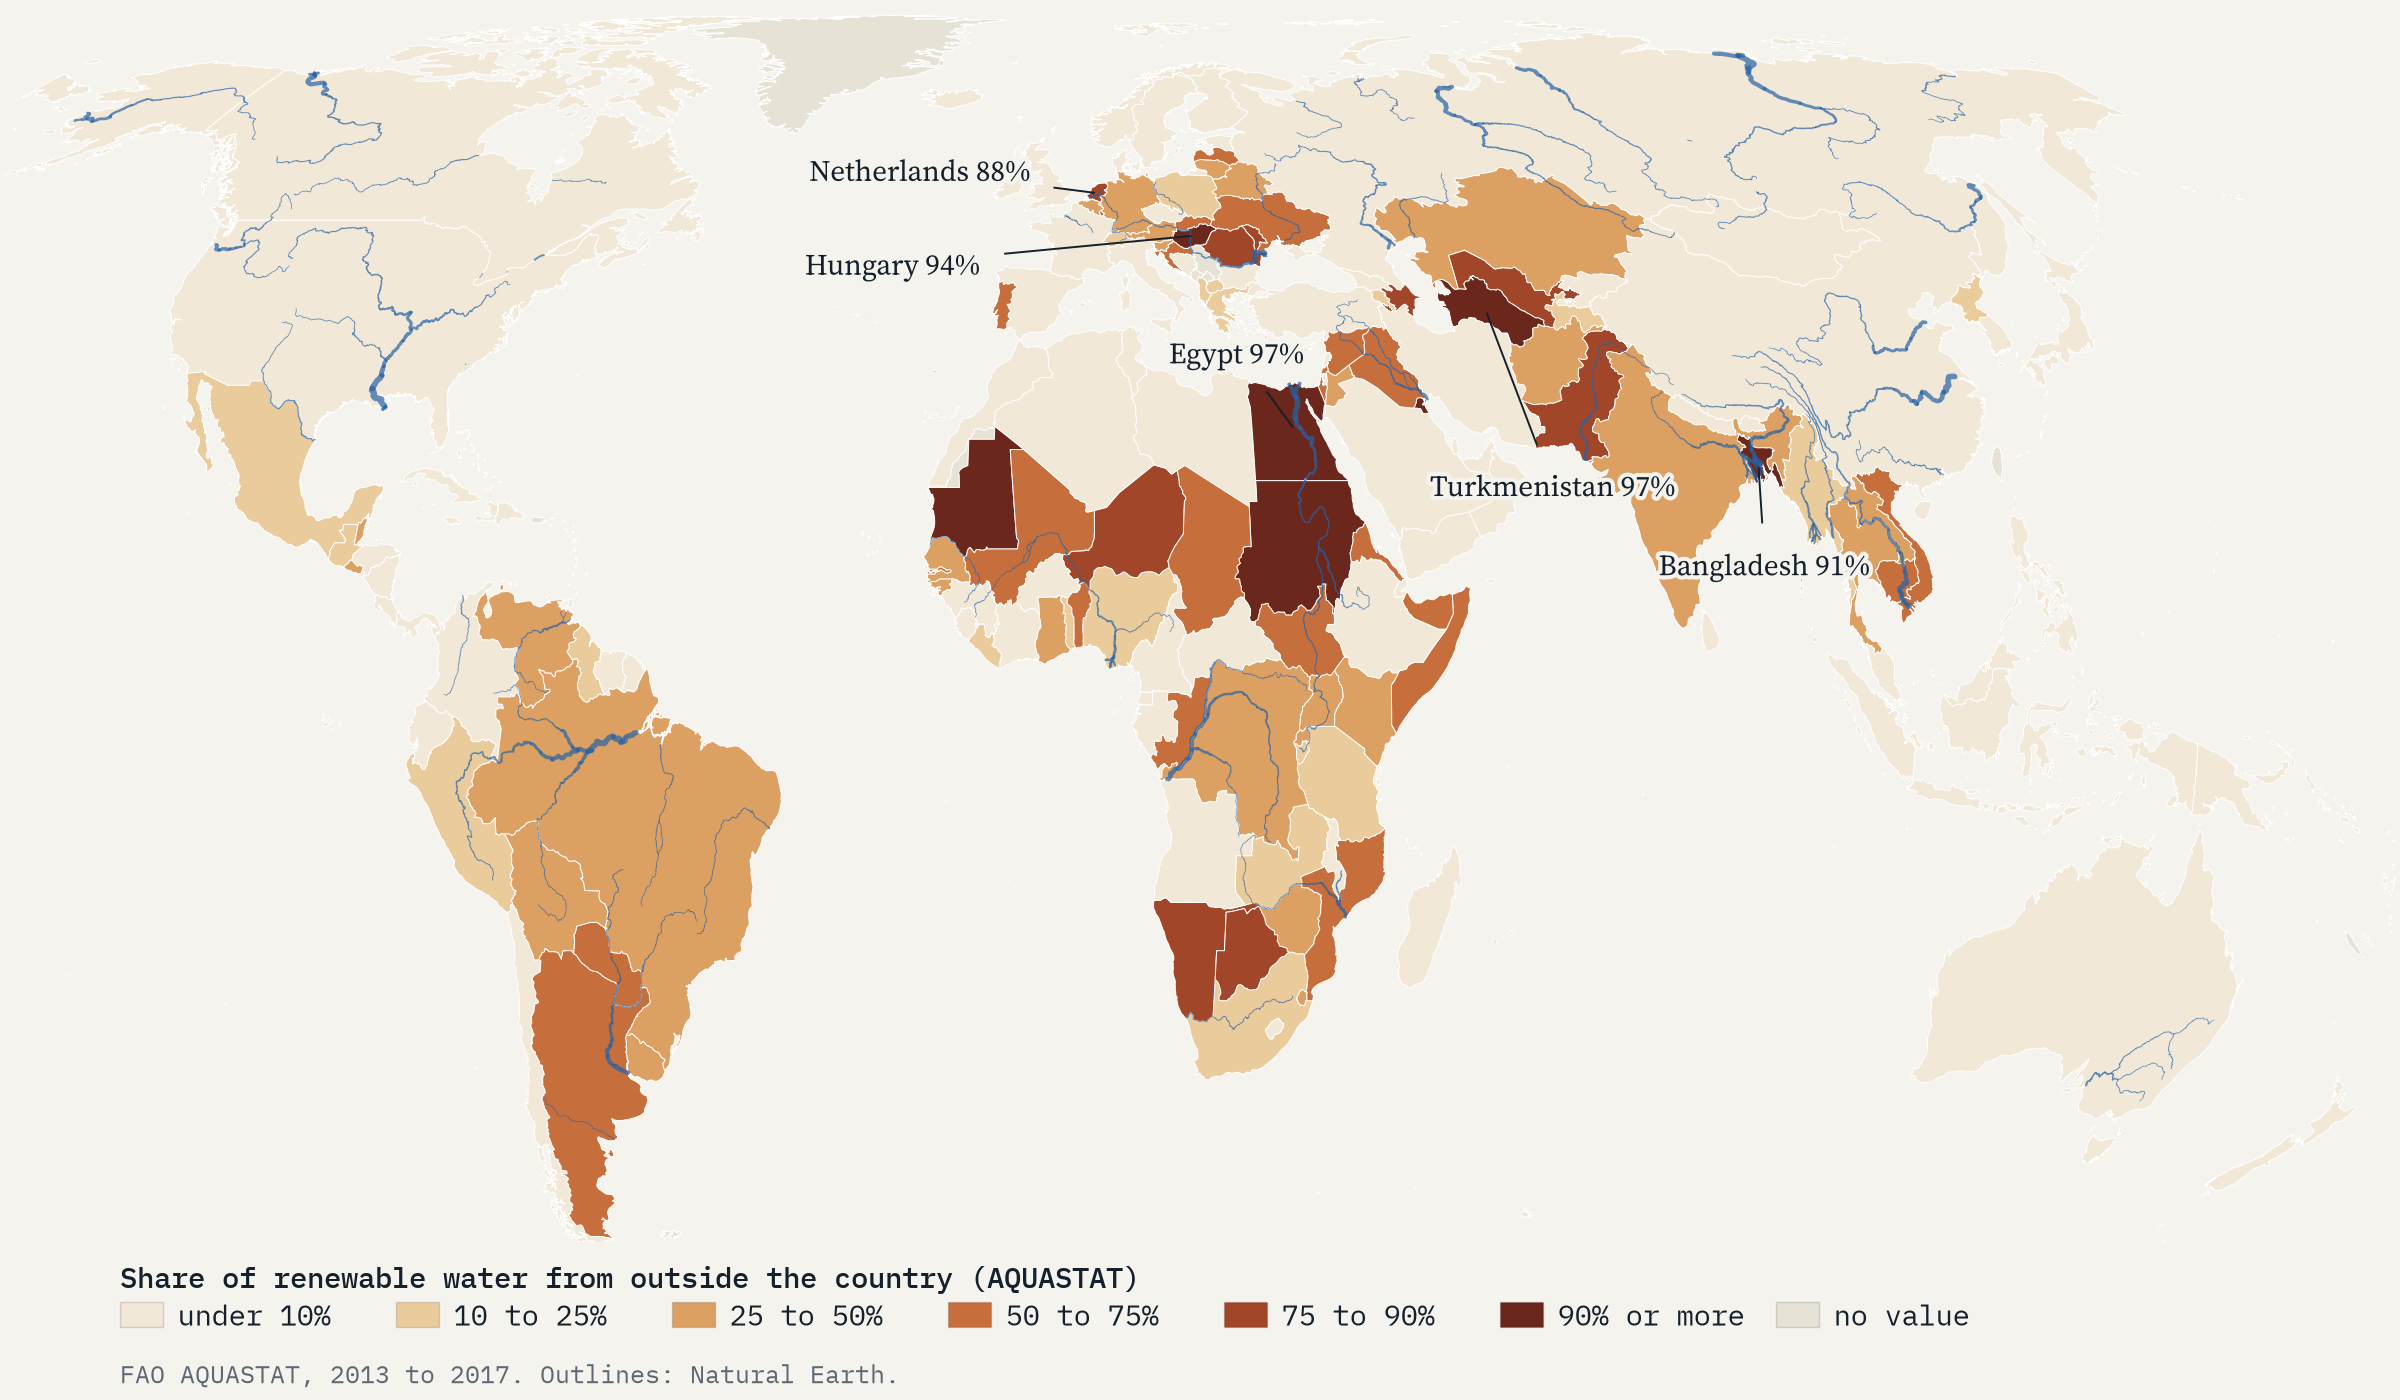
\includegraphics[width=\textwidth]{f_dependency.png}
\caption{AQUASTAT dependency ratio: the share of total renewable water resources originating outside the country, 2013 to 2017.}\label{fig:dep}\end{figure}

\begin{table}[tbp]\centering\small\caption{The highest AQUASTAT dependency ratios (\% of total renewable water resources originating outside the country), 2013 to 2017.}\label{tab:dep}\label{fig:depbars}\begin{tabular}{lr}\toprule Country & Dependency ratio (\%)\\\midrule
Kuwait & 100.0\\
Turkmenistan & 97.0\\
Egypt & 96.9\\
Bahrain & 96.5\\
Mauritania & 96.5\\
Sudan & 96.1\\
Hungary & 94.2\\
Bangladesh & 91.4\\
Niger & 89.7\\
Netherlands & 87.9\\
Moldova & 86.8\\
Namibia & 84.6\\
Botswana & 80.4\\
Uzbekistan & 80.1\\
Romania & 80.0\\
Pakistan & 77.7\\
\bottomrule\end{tabular}\end{table}

\section{Discussion}
The shared basin is the ordinary condition of the world's large rivers, not the exception. Nearly half the land outside Antarctica and nearly half of humanity sit in basins that cross a border. The distribution is skewed: hundreds of small basins are shared by two neighbours along a border, while a handful of great basins in Europe, Africa and Asia bring ten or more countries into one hydrological unit. How evenly the basin is divided matters as much as how many share it. The Danube's nineteen countries include several with tiny shares, while the Nile's eleven include upstream countries that provide much of its water and downstream countries that depend on it almost entirely.

The question of the longest river is a small lesson in measurement. Measured consistently on one map, the Nile is the longest system and the Amazon is third, behind the Yangtze, but the Amazon's position owes much to where Natural Earth draws its mouth, and the absolute lengths are not comparable with published ones at all. A ranking of river lengths is only as meaningful as the agreement on how they are measured, and no such agreement exists.

\section{Limitations}
First, the basin polygons are those of the 2018 spatial update, while the riparian lists and populations are from the 2024 table; three basins have no polygon. Second, counting countries depends on how disputed areas are treated, and other choices would give other counts (the TFDD itself lists 14 riparians for the Nile including disputed areas). Third, the river lengths are those of a generalised map: they are internally consistent but not survey lengths, and the matching of mouths, the joining tolerance and the exclusion of three linking channels all affect individual systems. Fourth, the countries along a river depend on the outlines and the buffer used, and short border stretches can be missed (Moldova on the Danube) or, near a border, counted. Fifth, the AQUASTAT values are a 2017 download of estimates for 2013 to 2017, and the dependency ratio combines surface water and groundwater. Sixth, the published lengths quoted are from one reference work and are themselves the product of choices. Finally, sharing a basin is not a measure of cooperation or conflict, which the TFDD records separately in its treaty and event databases.

\section{Conclusion}
Open data can map the world's shared rivers in detail: 313 basins, the share of each in each country, the rivers that drain them, and the countries whose water comes from upstream. The same data show why the longest river is a matter of definition. The atlas lets readers explore both.

\section*{Data and code availability}
The interactive atlas is at \url{https://maps.tristanhotham.com/shared-rivers/}. Data and code are at \url{https://github.com/Tristan-Hotham/shared-rivers} and archived with this paper at \texttt{10.5281/zenodo.23848927}. The TFDD files were taken from \url{https://github.com/hannahkfriedrich/tfdd} (2018 basins and basin country units) and \url{https://github.com/SharedWatersLab/geography} (2024 basin master table); the AQUASTAT table from \url{https://github.com/cmawer/pycon-2017-eda-tutorial}. Code is released under the MIT licence and text and figures under CC BY 4.0. Derived tables from the TFDD are shared for non-commercial research with credit to the TFDD, and the AQUASTAT column under CC BY-NC-SA 3.0 IGO.

\section*{AI statement}
I wrote the text, with drafting and editing assistance from Claude (Anthropic), which also helped prepare the analysis code. I reviewed and checked all text and results.

\begin{thebibliography}{12}
\bibitem[Britannica(2026a)]{brit_amazon} Encyclopaedia Britannica (2026) Amazon River. \url{https://www.britannica.com/place/Amazon-River}
\bibitem[Britannica(2026b)]{brit_nile} Encyclopaedia Britannica (2026) Nile River. \url{https://www.britannica.com/place/Nile-River}
\bibitem[Britannica(2026c)]{brit_yangtze} Encyclopaedia Britannica (2026) Yangtze River. \url{https://www.britannica.com/place/Yangtze-River}
\bibitem[Douglas and Peucker(1973)]{douglas1973} Douglas, D. H. and Peucker, T. K. (1973) Algorithms for the reduction of the number of points required to represent a digitized line or its caricature. \emph{Cartographica}, 10(2), 112 to 122.
\bibitem[FAO(2017)]{aquastat} FAO (2017) AQUASTAT: FAO's global information system on water and agriculture. Food and Agriculture Organization of the United Nations. CC BY-NC-SA 3.0 IGO. \url{https://www.fao.org/aquastat/}
\bibitem[Mandelbrot(1967)]{mandelbrot1967} Mandelbrot, B. (1967) How long is the coast of Britain? Statistical self-similarity and fractional dimension. \emph{Science}, 156(3775), 636 to 638.
\bibitem[Mawer(2017)]{pycon} Mawer, C. (2017) PyCon 2017 exploratory data analysis tutorial, AQUASTAT data. \url{https://github.com/cmawer/pycon-2017-eda-tutorial}
\bibitem[McCracken and Wolf(2019)]{mccracken2019} McCracken, M. and Wolf, A. T. (2019) Updating the Register of International River Basins of the world. \emph{International Journal of Water Resources Development}, 35(5), 732 to 782.
\bibitem[Natural Earth(2026)]{naturalearth} Natural Earth (2026) Rivers and lake centerlines (1:10m, scale ranks; 1:50m), lakes, land and admin 0 countries. Public domain. \url{https://www.naturalearthdata.com/}
\bibitem[TFDD(2024)]{tfdd} Transboundary Freshwater Dispute Database (2024) International River Basins. Oregon State University, College of Earth, Ocean, and Atmospheric Sciences. \url{https://transboundarywaters.ceoas.oregonstate.edu/}
\bibitem[Wolf et al.(1999)]{wolf1999} Wolf, A. T., Natharius, J. A., Danielson, J. J., Ward, B. S. and Pender, J. K. (1999) International river basins of the world. \emph{International Journal of Water Resources Development}, 15(4), 387 to 427.
\bibitem[World Bank(2026)]{wb} World Bank (2026) World Development Indicators: population, total (SP.POP.TOTL). CC BY 4.0. \url{https://data.worldbank.org/indicator/SP.POP.TOTL}
\end{thebibliography}
\end{document}
